\begin{abstract}
Ce mémoire présente la conception et la validation d'une architecture de sécurité \textit{Zero Trust}, conforme au NIST SP 800-207, pour les API bancaires ouvertes dans le contexte de l'Open Banking et de la directive PSD2. La solution intègre une passerelle NGINX utilisant mTLS, un serveur d'identité Keycloak reposant sur OAuth 2.0 et des jetons signés avec RS256, un backend FastAPI, un frontend Flask ainsi qu'une pile SIEM/SOAR réactive calculant un score dynamique de menace $T_{decay}(x, t)$. L'audit DAST réalisé avec OWASP ZAP n'a révélé aucune vulnérabilité critique dans le périmètre évalué. Les tests de performance ont mesuré un surcoût de 34,1~ms, portant la latence totale à 72,3~ms, soit une valeur nettement inférieure au seuil SLA de 200~ms.
\end{abstract}

\section*{Présentation générale du projet}
Ce projet propose une architecture robuste pour répondre aux défis de l'Open Banking. Il associe une barrière cryptographique au niveau de la couche transport (mTLS) à un mécanisme de défense active (SOAR), capable d'isoler une adresse IP hostile en moins de 30 secondes. L'ensemble a été validé au moyen d'un prototype conteneurisé sous Docker.

\subsection*{Langue de rédaction}
Ce mémoire est rédigé en langue française conformément aux normes de l'ISIMG. Les termes techniques et acronymes anglophones consacrés (API, mTLS, JWT, RBAC, SIEM, SOAR, DAST) sont conservés dans leur forme originale et définis dès leur première apparition.

% ============================================================
\section{Introduction générale et état de l'art}
% ============================================================

La transformation numérique du secteur bancaire, impulsée par l'adoption de la directive européenne sur les services de paiement (PSD2 / DSP2) \cite{psd2}, a conduit les institutions financières à ouvrir leurs systèmes d'information à des prestataires tiers agréés (\textit{Third Party Providers} -- TPP). Ces prestataires, qui interviennent comme fournisseurs de services d'information sur les comptes (AISP) ou comme prestataires de services d'initiation de paiement (PISP), interagissent directement avec les interfaces de programmation applicative (API) bancaires. Si cette ouverture favorise l'interopérabilité et l'innovation financière, elle accroît également l'exposition des systèmes bancaires aux cybermenaces.

\subsection{Contexte et problématique de la sécurité bancaire ouverte}
La sécurisation des API financières se heurte à un changement de paradigme : l'effacement de la frontière périmétrique traditionnelle de l'entreprise. Les modèles de sécurité conventionnels reposent sur une défense de type « château fort » (pare-feux, zones démilitarisées et réseaux locaux implicitement réputés sûrs) et supposent que les flux internes sont dignes de confiance. Dans le contexte de l'Open Banking, où des applications tierces hétérogènes accèdent à des ressources sensibles, cette hypothèse de confiance implicite n'est plus adaptée.

Les dispositifs traditionnels présentent deux écueils majeurs :
\begin{itemize}[leftmargin=*]
    \item \textbf{Les limites des pare-feux applicatifs conventionnels (WAF)} : Les WAF analysent principalement les flux à l'aide de signatures statiques et d'expressions régulières. S'ils sont efficaces contre des attaques classiques, telles que les injections SQL ou les scripts intersites (XSS), ils sont moins adaptés à la détection des abus de logique métier, comme la manipulation d'identifiants dans une attaque BOLA, ou de certaines usurpations de session.
    \item \textbf{La passivité des systèmes SIEM traditionnels} : Les plateformes de gestion des événements et des informations de sécurité (SIEM), telles que la pile ELK ou Splunk, collectent et indexent des volumes considérables de journaux. Toutefois, leur utilisation traditionnelle demeure principalement orientée vers l'analyse après incident ou l'émission d'alertes destinées aux opérateurs du SOC. Face à des attaques automatisées et rapides, le délai d'intervention humaine peut s'avérer insuffisant.
\end{itemize}

\subsection{Standards d'identité et de sécurité financière (FAPI, OAuth 2.0, mTLS)}
Pour encadrer techniquement l'ouverture des API, l'industrie financière et les organismes de normalisation ont établi des référentiels exigeants :
\begin{itemize}[leftmargin=*]
    \item \textbf{Financial-grade API (FAPI 1.0 Advanced)} \cite{fapi} : Spécification émise par l'OpenID Foundation durcissant OAuth 2.0 pour les environnements à haut risque financier. Elle requiert l'authentification mutuelle TLS (mTLS), l'association cryptographique des jetons aux certificats clients (\textit{Certificate-Bound Access Tokens}) et l'usage de PKCE.
    \item \textbf{OAuth 2.0 (RFC 6749) et OpenID Connect (OIDC)} \cite{oauth2} : Protocoles de délégation d'autorisation et d'authentification permettant à un utilisateur d'accorder à un TPP un accès restreint à ses comptes sans lui transmettre ses identifiants bancaires.
    \item \textbf{Mutual TLS (RFC 8705)} \cite{rfc8705} : Authentification mutuelle au niveau de la couche transport (TLS) où le client TPP et la passerelle d'API NGINX présentent chacun un certificat cryptographique validé.
    \item \textbf{JSON Web Token (JWT - RFC 7519)} \cite{rfc7519} : Format de jeton compact et auto-contenu, signé numériquement par Keycloak au moyen de l'algorithme asymétrique RS256, permettant une validation d'intégrité et de portée (\textit{scope}) par le backend API sans requête systématique à la base de données.
\end{itemize}

\subsection{Le modèle de sécurité Zero Trust (NIST SP 800-207)}
Face à la dissolution du périmètre, notre démarche opérationnalise les sept principes fondamentaux de l'architecture \textit{Zero Trust} définie par le NIST dans la publication spéciale SP 800-207 \cite{nist_zt} :
\begin{enumerate}[leftmargin=*]
    \item Toutes les sources de données et services de calcul sont considérés comme des ressources discrètes à protéger.
    \item L'ensemble des communications réseau est sécurisé, indépendamment de l'emplacement physique ou logique du client.
    \item L'accès aux ressources individuelles est concédé sur une base par session, avec le principe du moindre privilège.
    \item L'autorisation d'accès est gouvernée par une politique dynamique combinant identité vérifiée, état de l'application et comportement observé.
    \item L'organisation surveille en continu l'intégrité et la posture de sécurité de tous les actifs associés.
    \item L'authentification et l'autorisation sont strictement exigées et vérifiées avant tout octroi d'accès.
    \item L'organisation collecte et analyse en permanence des données contextuelles sur l'état des communications pour affiner dynamiquement sa posture défensive.
\end{enumerate}

\subsection{De la supervision SIEM passive à la réponse active automatisée (SOAR)}
L'innovation centrale de ce travail repose sur le couplage d'un système de journalisation et d'ingestion (pile ELK) avec un moteur de décision réactif intégré au middleware de l'API. Cette synergie transforme la supervision passive en un automate de réponse active (\textit{Security Orchestration, Automation and Response} -- SOAR). Dès la détection d'un comportement hostile caractérisé par un franchissement de seuil de menace, le système applique de façon autonome un blocage applicatif temporaire de l'adresse IP source, tout en notifiant l'analyste de sécurité via un canal temps réel (Server-Sent Events).

\clearpage
% ============================================================
\section{Spécification du Système et Analyse des Menaces}
% ============================================================

\subsection{Périmètre fonctionnel et services bancaires ouverts}
Le démonstrateur bancaire implémente les services fondamentaux exigés dans le cadre d'un système d'Open Banking moderne :
\begin{itemize}[leftmargin=*]
    \item Consultation des soldes et historique des écritures comptables (AISP).
    \item Initiation de virements ponctuels et programmés entre comptes (PISP).
    \item Gestion du carnet de bénéficiaires de confiance.
    \item Consultation des crédits en cours et suivi budgétaire.
    \item Gestion du cycle de vie des consentements accordés aux applications tierces (TPP).
\end{itemize}

\subsection{Cartographie des acteurs, des actifs sensibles et des frontières de confiance}
L'écosystème comprend trois catégories d'acteurs distincts :
\begin{enumerate}[leftmargin=*]
    \item \textbf{Propriétaire de la ressource (client bancaire)} : Titulaire légitime des comptes, qui interagit avec le système au moyen du portail frontend ou accorde des autorisations précises à des applications tierces.
    \item \textbf{Client OAuth / TPP (prestataire tiers)} : Entité logicielle externe agréée qui accède aux API après l'établissement d'une connexion mTLS et l'obtention du consentement du client.
    \item \textbf{Administrateur de la sécurité (analyste SOC)} : Opérateur chargé de surveiller le tableau de bord des alertes, de gérer la liste blanche et d'examiner les incidents de sécurité.
\end{enumerate}

Les actifs sensibles à protéger comprennent les identifiants et les clés cryptographiques stockés dans PostgreSQL et Keycloak, les données financières conservées dans MongoDB, les clés privées associées aux certificats TLS de la banque ainsi que les journaux de sécurité. Les frontières de confiance (\textit{Trust Boundaries}) séparent l'Internet externe, la zone démilitarisée (\texttt{dmz-net}), la zone applicative (\texttt{backend-tier}), le réseau de persistance (\texttt{data-tier}) et la zone de surveillance (\texttt{monitoring-tier}).

\subsection{Exigences fonctionnelles, non-fonctionnelles et sécuritaires}
\begin{itemize}[leftmargin=*]
    \item \textbf{Exigences fonctionnelles} : Exécution conforme des flux financiers, gestion granulaire des consentements et visualisation continue des alertes de sécurité.
    \item \textbf{Exigences sécuritaires} : Authentification forte du client (SCA), authentification mutuelle transport (mTLS) pour les TPP, cloisonnement réseau strict par conteneurs, non-répudiation des opérations via des journaux à altération détectable.
    \item \textbf{Exigences de performance} : Temps de réponse moyen maintenu sous le seuil contractuel de 200~ms (SLA bancaire) et délai de déclenchement du blocage applicatif inférieur à 30 secondes.
\end{itemize}

\subsection{Modélisation des cas d'utilisation}
La Figure~\ref{fig:global_uc} expose le diagramme des cas d'utilisation du système bancaire sécurisé, en distinguant clairement les opérations réservées aux utilisateurs finaux et administrateurs du parcours d'accès délégué des partenaires TPP.

\begin{figure}[H]
    \centering
    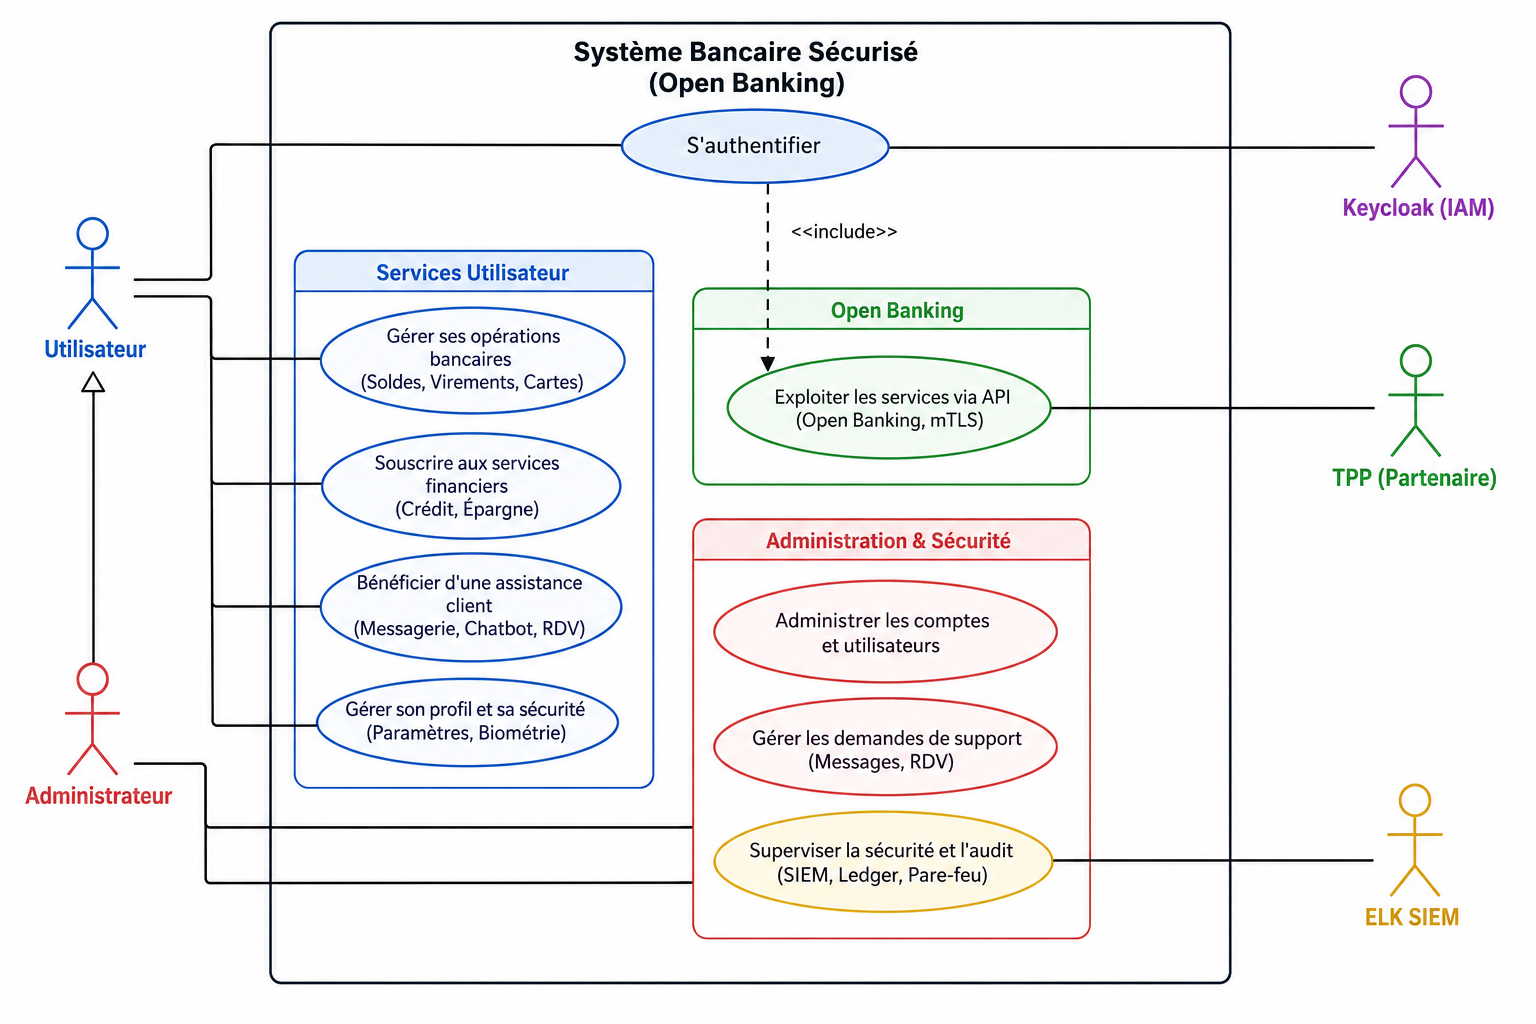
\includegraphics[width=1\linewidth]{uploads/global_uc_diagram.png}
    \caption{Diagramme des cas d'utilisation du système bancaire sécurisé.}
    \label{fig:global_uc}
\end{figure}

Comme l'illustre la Figure~\ref{fig:global_uc}, l'accès aux services métiers (comptes, virements, consentements) et aux fonctionnalités de supervision (gestion des alertes, blocage IP) est structuré selon des rôles bien définis, évitant les inclusions systématiques superflues et séparant le flux de support administratif du flux bancaire nominal.

\scenariotable
{Interaction globale avec le système bancaire}
{Client, Administrateur, TPP}
{Permettre l'accès aux services bancaires tout en assurant une surveillance en continu et une isolation hermétique.}
{L'infrastructure conteneurisée est déployée et les services IAM et SIEM sont opérationnels.}
{L'opération financière ou administrative est exécutée et consignée dans le journal d'audit.}
{1. L'utilisateur ou le TPP transmet sa requête. 2. La passerelle NGINX valide TLS/mTLS. 3. Le backend FastAPI vérifie le jeton JWT et la portée requise. 4. Le service métier traite la demande et enregistre l'événement.}
{En cas d'échec de vérification ou de comportement hostile, l'événement est capturé par le middleware d'audit, le score de menace est incrémenté et une alerte SSE est transmise au tableau de bord.}
{Traçabilité totale, conformité aux exigences PSD2/SCA.}

\scenariotable
{Gestion des consentements Open Banking (TPP)}
{Client bancaire, Application TPP, Serveur Keycloak}
{Accorder une délégation d'accès temporaire et restreinte à un TPP pour la consultation de comptes.}
{Le client possède un compte actif et l'application TPP est authentifiée par certificat mTLS auprès de NGINX.}
{Le consentement est enregistré et Keycloak délivre un jeton d'accès délimité au TPP.}
{1. Le TPP redirige le navigateur du client vers Keycloak. 2. Le client s'authentifie avec son second facteur. 3. Le client valide les portées demandées. 4. Keycloak crée l'entité Consent et génère le code d'autorisation.}
{Si le client refuse ou si la portée sollicitée est invalide, Keycloak renvoie un refus d'autorisation au TPP et aucun jeton n'est généré.}
{Révocabilité immédiate du consentement et principe du moindre privilège.}

\scenariotable
{Blocage applicatif automatique d'une adresse IP suspecte}
{Threat Monitor, SecurityState, Administrateur SIEM}
{Isoler de manière autonome une adresse IP source émettant des requêtes malveillantes répétées.}
{Le middleware de sécurité consigne les erreurs HTTP (401, 403, 429) dans le journal d'audit.}
{L'adresse IP est inscrite dans le registre des adresses bloquées et ses requêtes futures sont rejetées (code 403).}
{1. L'attaquant envoie des requêtes abusives. 2. Le Threat Monitor calcule le score $T_{decay}(x,t)$. 3. Le score dépasse le seuil critique $S=3.0$. 4. Une alerte CRITICAL est émise via SSE. 5. Un minuteur de 30s s'active. 6. À expiration, SecurityState bloque l'adresse IP.}
{L'administrateur annule manuellement le blocage sur le tableau de bord avant la fin du minuteur en cas de faux positif identifié.}
{Découplage asynchrone pour ne pas impacter la latence des flux légitimes.}

\subsection{Analyse formelle des menaces (STRIDE)}
L'évaluation méthodique de la résilience du système a été menée au moyen de la méthode de modélisation des menaces STRIDE \cite{stride_model}. Le Tableau~\ref{tab:stride} récapitule les six catégories de menaces identifiées, leur portée technique et les contre-mesures architecturales mises en œuvre dans le cadre de ce projet.

\begin{table}[H]
    \centering
    \footnotesize
    \begin{tabular}{|>{\raggedright\arraybackslash}p{0.20\linewidth}|>{\raggedright\arraybackslash}p{0.31\linewidth}|>{\raggedright\arraybackslash}p{0.41\linewidth}|}
        \hline
        \textbf{Menace STRIDE} & \textbf{Définition} & \textbf{Contre-mesure mise en œuvre} \\ \hline
        \textbf{S}poofing & Usurpation d'identité d'un client ou d'un TPP & Authentification mutuelle mTLS (certificats X.509 privés) et jetons JWT signés en RS256 par Keycloak. \\ \hline
        \textbf{T}ampering & Altération non autorisée des données en transit & Chiffrement systématique TLS 1.3 et validation cryptographique des signatures de jetons. \\ \hline
        \textbf{R}epudiation & Répudiation d'une action financière ou d'administration & Traçabilité multicouche par journaux à altération détectable (format JSONL append-only horodaté) et indexation Elasticsearch. \\ \hline
        \textbf{I}nformation Disclosure & Divulgation de données confidentielles & Cloisonnement des réseaux Docker, validation stricte des schémas Pydantic et masquage du PAN. \\ \hline
        \textbf{D}enial of Service & Déni de service et saturation des ressources & Régulation de débit multicouche (NGINX \textit{rate limiting} et SlowAPI) couplée au blocage applicatif dynamique. \\ \hline
        \textbf{E}levation of Privilege & Élévation non autorisée de privilèges & Contrôle d'accès basé sur les rôles (RBAC) et validation stricte des portées OAuth2 (\textit{scopes}). \\ \hline
    \end{tabular}
    \caption{Modélisation des menaces STRIDE et contre-mesures de sécurité associées.}
    \label{tab:stride}
\end{table}

L'examen du Tableau~\ref{tab:stride} met en évidence que chaque vecteur de menace trouve une contre-mesure technique vérifiable au sein de l'infrastructure, assurant une protection globale conforme aux recommandations de la norme ISO/IEC 27001 \cite{iso27001}.

\clearpage
% ============================================================
\section{Architecture et Conception Technique}
% ============================================================

Notre conception met en pratique le principe fondamental de la \textbf{défense en profondeur}, articulé autour de deux paliers complémentaires : la barrière d'accès et d'identité (NGINX, Keycloak, FastAPI, Flask) et le dispositif de surveillance et de réaction (pile ELK, Threat Monitor, SecurityState).

\subsection{Architecture globale et segmentation réseau Zero Trust}
La Figure~\ref{fig:deployment} présente l'architecture de déploiement sécurisée du système avec isolation réseau stricte.

\begin{figure}[H]
    \centering
    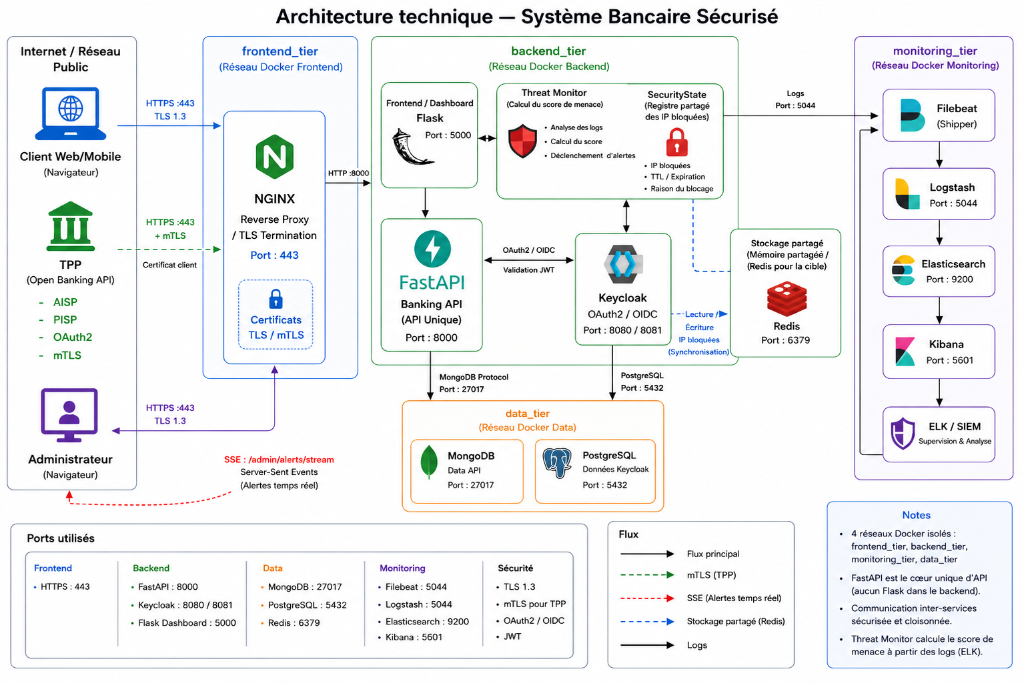
\includegraphics[width=1\linewidth]{uploads/DeploymentArchitecture.drawio.png}
    \caption{Architecture de déploiement sécurisée et segmentation réseau Zero Trust.}
    \label{fig:deployment}
\end{figure}

Comme le met en évidence la Figure~\ref{fig:deployment}, l'infrastructure est cloisonnée en quatre réseaux virtuels isolés :
\begin{itemize}[leftmargin=*]
    \item \textbf{Zone Frontière (DMZ / \texttt{frontend\_tier})} : La passerelle NGINX constitue l'unique point d'entrée exposé sur les ports 80 (redirection HTTPS) et 443. Elle réalise la terminaison TLS, le contrôle strict des certificats mTLS pour les partenaires TPP et applique la première couche de limitation de débit.
    \item \textbf{Zone Applicative (\texttt{backend\_tier})} : Réseau interne abritant le serveur backend FastAPI (port 8000), le serveur frontend/tableau de bord Flask (port 5000), le serveur d'identité Keycloak (ports 8080 / 8081), ainsi que les composants internes de sécurité \textit{ThreatMonitor} (calcul du score de menace), \textit{SecurityState} (registre des adresses IP bloquées avec synchronisation) et le stockage partagé (\textit{Redis} sur le port 6379 pour l'architecture cible). Aucun de ces services n'est accessible directement depuis l'extérieur sans traverser NGINX.
    \item \textbf{Cœur de Données (\texttt{data\_tier})} : Sous-réseau à connectivité interne exclusive (\texttt{internal: true}), hébergeant la base MongoDB (port 27017 pour les données financières) et la base PostgreSQL (port 5432 pour les métadonnées Keycloak).
    \item \textbf{Zone de Surveillance (\texttt{monitoring\_tier})} : Réseau dédié à la supervision de sécurité, interconnectant Filebeat (port 5044), Logstash (port 5044), Elasticsearch (port 9200) et Kibana (port 5601).
\end{itemize}

\subsection{Modèle d'identité, d'habilitation et flux d'accès TPP}
La passerelle NGINX authentifie les applications tierces (TPP) au moyen de certificats de test émis par une autorité privée (CA interne de la banque). La Figure~\ref{fig:seq_tpp} détaille la séquence d'accès Open Banking d'un TPP mettant en jeu le protocole Authorization Code avec mTLS.

\begin{figure}[H]
    \centering
    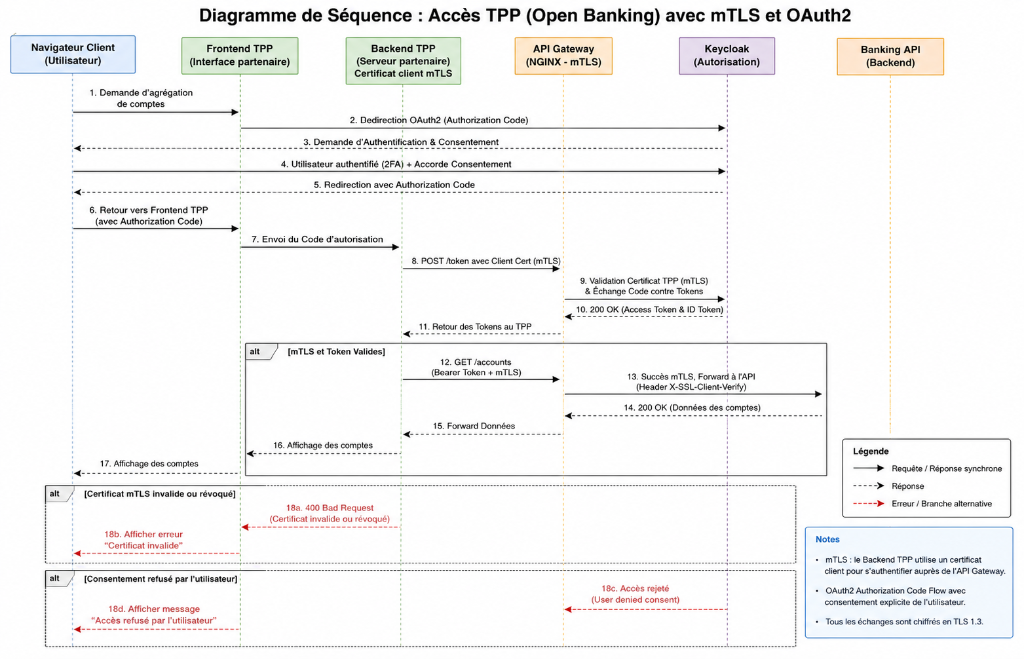
\includegraphics[width=1\linewidth]{uploads/sequence_open_banking_tpp.drawio.png}
    \caption{Séquence d'accès Open Banking via TPP avec authentification mTLS et flux d'autorisation.}
    \label{fig:seq_tpp}
\end{figure}

L'analyse de la séquence présentée en Figure~\ref{fig:seq_tpp} montre que la connexion mTLS est validée avant toute communication applicative. La séquence distingue trois entités côté TPP : le navigateur du client final (qui effectue la redirection d'autorisation), le frontend du TPP (interface web) et le backend du TPP (serveur qui échange le code d'autorisation contre le jeton). Ce découplage est essentiel pour la conformité FAPI : seul le backend, qui détient la clé privée mTLS, communique directement avec l'API bancaire. Le TPP redirige le navigateur du client vers Keycloak avec les paramètres \texttt{state}, \texttt{nonce}, \texttt{code\_challenge} (PKCE) et les portées souhaitées (\texttt{accounts:read}, \texttt{payments:write}). Après authentification forte du client et enregistrement explicite du consentement, Keycloak délivre un code d'autorisation échangé par le backend du TPP contre un jeton JWT RS256. En cas d'échec à l'une des étapes (certificat mTLS invalide, consentement refusé, portée non autorisée ou jeton expiré), la passerelle ou Keycloak retourne un code d'erreur HTTP approprié (400, 401 ou 403) et l'événement est consigné dans le journal d'audit.

\scenariotable
{Parcours d'accès TPP Open Banking avec mTLS}
{Navigateur Client, Backend TPP, NGINX Gateway, Keycloak, Backend FastAPI}
{Délivrer un accès sécurisé aux ressources bancaires à un tiers de confiance dûment authentifié.}
{Le TPP dispose d'une clé privée et d'un certificat émis par la CA privée de la banque.}
{Le TPP obtient un jeton JWT valide et accède aux données d'information sur les comptes.}
{1. NGINX valide le certificat mTLS du TPP. 2. Le client s'authentifie et accorde son consentement sur Keycloak. 3. Le TPP échange le code d'autorisation contre un JWT. 4. Le TPP consomme l'API FastAPI avec le JWT.}
{En cas de certificat mTLS révoqué, de portée non consentie ou de jeton expiré, la passerelle ou l'API retourne un code d'erreur (400, 401 ou 403) et notifie le système de journalisation.}
{Conformité FAPI 1.0 Advanced et validation sans état des jetons.}

Le modèle de classes du système d'identité et de gestion des accès (IAM) est modélisé dans la Figure~\ref{fig:iam_class}.

\begin{figure}[H]
    \centering
    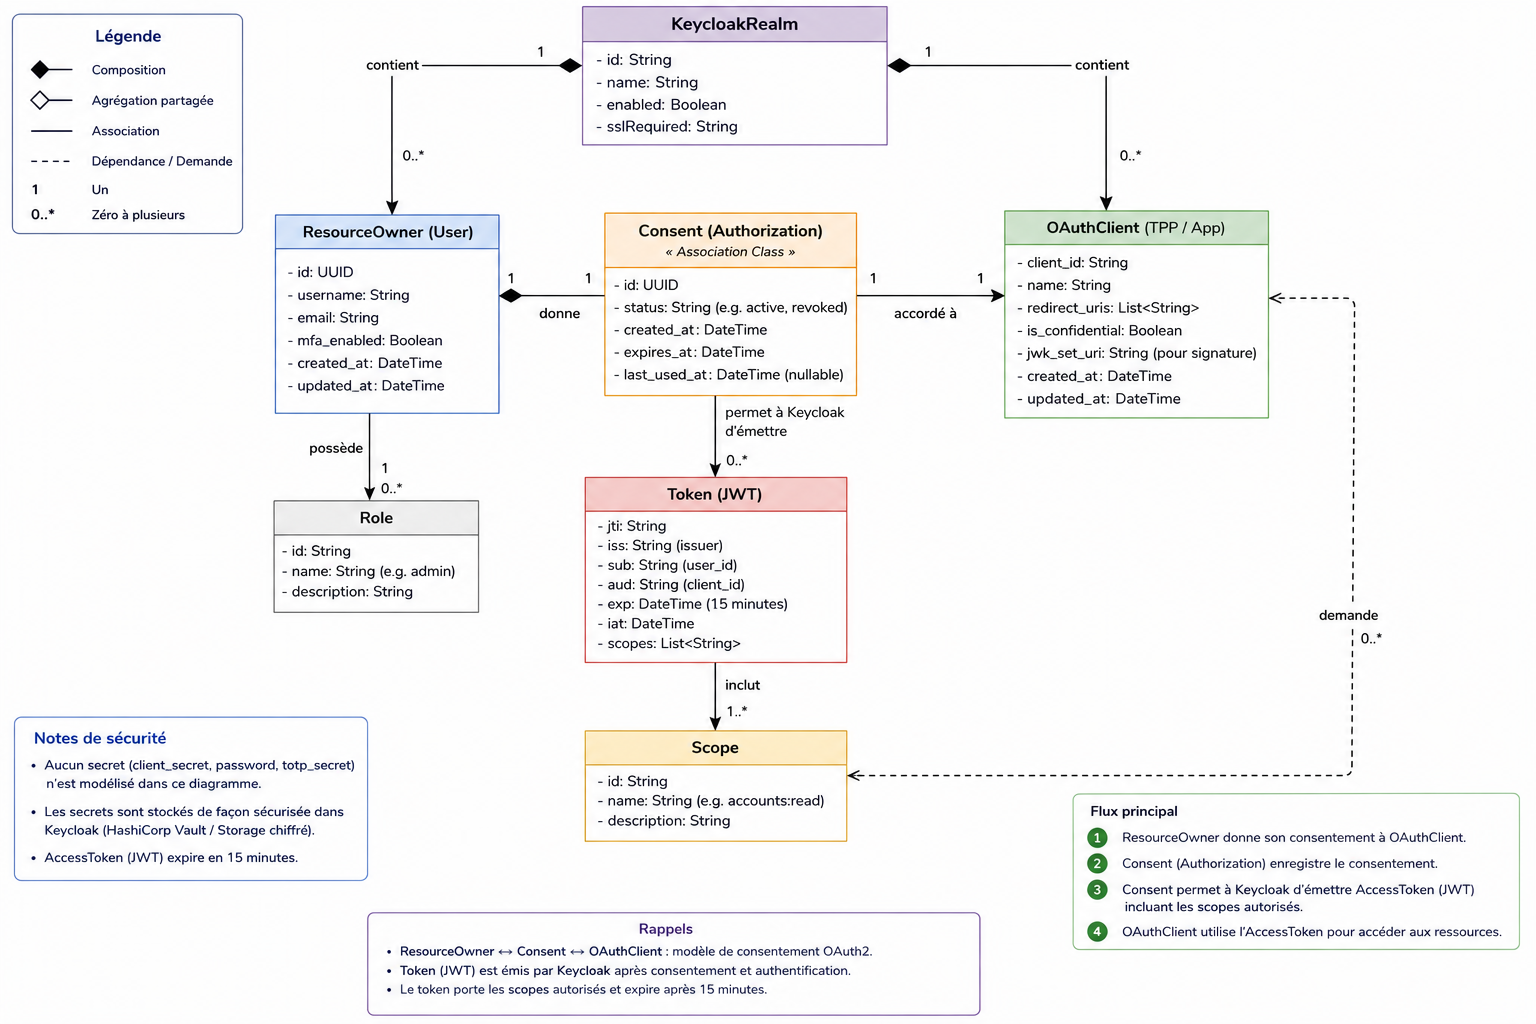
\includegraphics[width=1\linewidth]{uploads/classIAM.drawio.png}
    \caption{Modèle de données IAM et relations de consentement Open Banking.}
    \label{fig:iam_class}
\end{figure}

Comme explicité dans la Figure~\ref{fig:iam_class}, le modèle dissocie rigoureusement l'identité de l'utilisateur (\textit{ResourceOwner}) de l'application cliente tierce (\textit{OAuthClient}). L'entité \textit{Consent} matérialise l'association entre le propriétaire des données et le client OAuth pour une liste définie de portées (\textit{Scope}), avec date de création et d'expiration. Les secrets sensibles (mots de passe hachés, clés privées, secrets clients) sont confinés au sein du référentiel sécurisé de Keycloak et n'apparaissent pas en clair dans le modèle de domaine métier.

Le processus d'authentification forte à double facteur (2FA) des utilisateurs humains est illustré par la Figure~\ref{fig:seq_2fa}.

\begin{figure}[H]
    \centering
    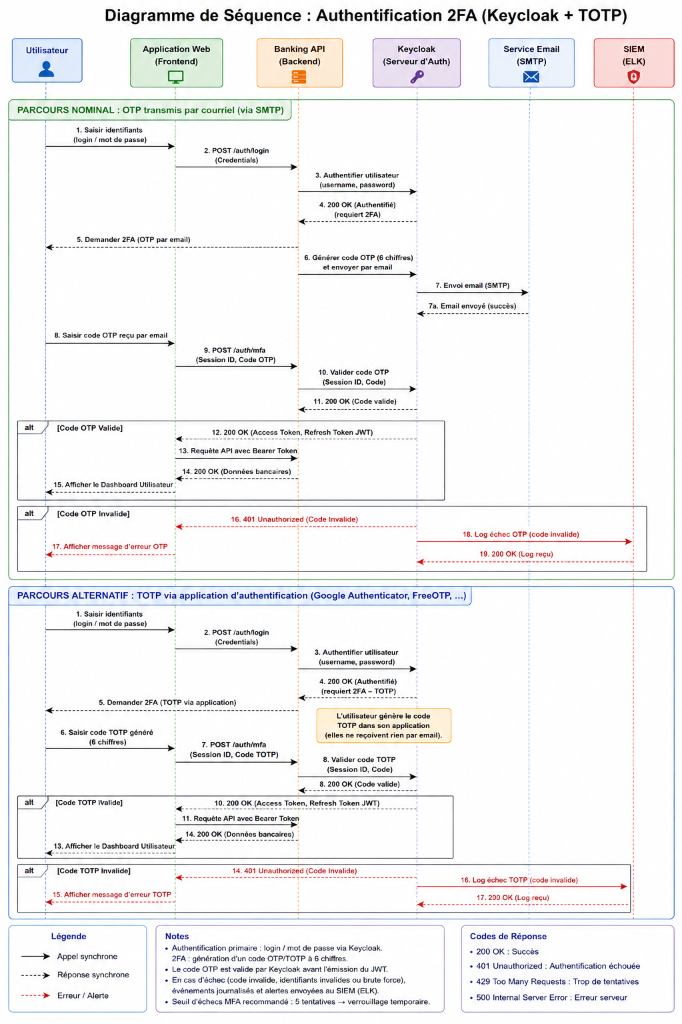
\includegraphics[width=1\linewidth]{uploads/seq_auth2.drawio.png}
    \caption{Processus d'authentification forte (2FA) : parcours OTP par courriel (nominal) et TOTP (alternatif).}
    \label{fig:seq_2fa}
\end{figure}

L'enchaînement décrit par la Figure~\ref{fig:seq_2fa} démontre que l'accès utilisateur exige la validation successive de deux facteurs distincts. Le premier facteur est le mot de passe principal (facteur de connaissance), intégralement géré et haché par Keycloak --- aucun attribut \texttt{password\_hash} n'est stocké dans le modèle de domaine métier de l'application. Le second facteur (facteur de possession) est implémenté selon deux parcours exclusifs : \textbf{(a) OTP par courriel} (parcours nominal) : Keycloak génère un code à usage unique à 6 chiffres transmis via SMTP au client, valable 5 minutes ; \textbf{(b) TOTP} (parcours alternatif) : le client enregistre une application d'authentification (Google Authenticator, FreeOTP) et génère un code RFC 6238 renouvelé toutes les 30 secondes. Les deux options sont configurables individuellement par compte dans Keycloak. Pour l'option d'authentification biométrique proposée au niveau du portail frontend, le gabarit facial est analysé localement avec contrôle de vivacité (\textit{liveness detection}) pour se prémunir des attaques par rejeu, avec bascule systématique vers la procédure nominale (mot de passe + OTP) en cas d'échec.

\scenariotable
{Authentification forte de l'utilisateur (2FA)}
{Utilisateur, Frontend Flask, Serveur Keycloak, Service SMTP}
{Valider l'identité du client bancaire conformément aux exigences SCA de la directive PSD2.}
{L'utilisateur possède un compte actif et une adresse électronique vérifiée (parcours OTP) ou une application TOTP enregistrée (parcours alternatif).}
{L'utilisateur reçoit un jeton d'accès JWT et un jeton de rafraîchissement (\textit{Refresh Token}).}
{1. L'utilisateur saisit son identifiant et mot de passe (validé par Keycloak). 2a. (Parcours OTP) Le système génère un code OTP transmis par courriel. 2b. (Parcours TOTP) L'utilisateur consulte son application d'authentification. 3. L'utilisateur saisit le code éphémère valide. 4. Les jetons de session sont émis.}
{En cas de code erroné ou expiré, la tentative est rejetée, l'échec est tracé dans le journal Keycloak et le compteur d'échecs est incrémenté.}
{Rotation systématique des jetons de rafraîchissement et expiration courte du jeton d'accès (15 minutes).}

\subsection{Modèle de données bancaire sécurisé}
Le modèle de données de l'application bancaire est représenté sur la Figure~\ref{fig:global_class}.

\begin{figure}[H]
    \centering
    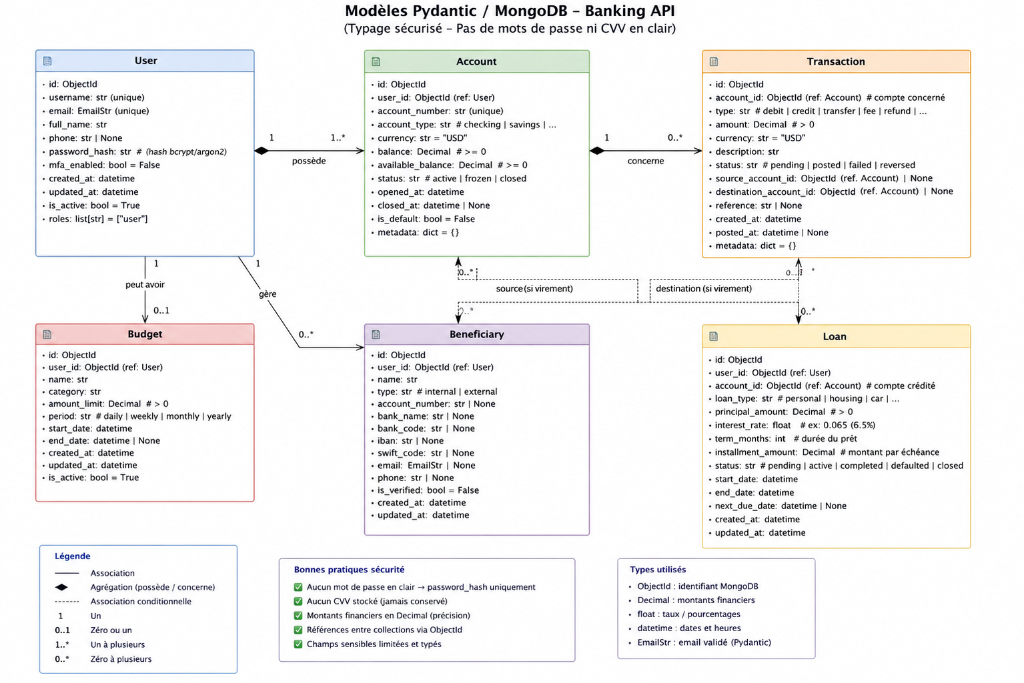
\includegraphics[width=1\linewidth]{uploads/global_class_diagram.png}
    \caption{Modèle de données global de l'application bancaire.}
    \label{fig:global_class}
\end{figure}

L'examen de la Figure~\ref{fig:global_class} illustre les règles de conception appliquées pour préserver l'intégrité et la confidentialité des données financières :
\begin{itemize}[leftmargin=*]
    \item \textbf{Précision monétaire (\texttt{Decimal})} : Les montants des entités \textit{Account}, \textit{Transaction}, \textit{Budget} et \textit{Loan} utilisent le type à virgule fixe \texttt{Decimal}, excluant tout risque d'imprécision d'arrondi inhérent aux types flottants standard.
    \item \textbf{Typage strict et validation Pydantic} : Les champs sensibles et les adresses électroniques sont contrôlés à l'ingestion via \texttt{EmailStr} et les liaisons inter-collections s'effectuent par identifiants \texttt{ObjectId} uniques.
    \item \textbf{Protection des secrets et conformité PCI-DSS} : Aucun mot de passe n'est stocké en clair (seul un condensat haché sous \texttt{bcrypt}/\texttt{argon2} est conservé), et les codes de sécurité de cartes (CVV) ne sont jamais persistés en base de données.
    \item \textbf{Modélisation complète du domaine bancaire} : Les flux monétaires (\textit{Transaction}), les plafonds de dépenses (\textit{Budget}), le carnet de tiers de confiance (\textit{Beneficiary}) et les échéances de crédit (\textit{Loan}) sont structurés selon des schémas explicites et modulaires.
\end{itemize}

\subsection{Architecture du SIEM et module de réponse active}
La Figure~\ref{fig:class_siem} expose le diagramme de classes des composants de journalisation, d'analyse de menace et de réponse active.

\begin{figure}[H]
    \centering
    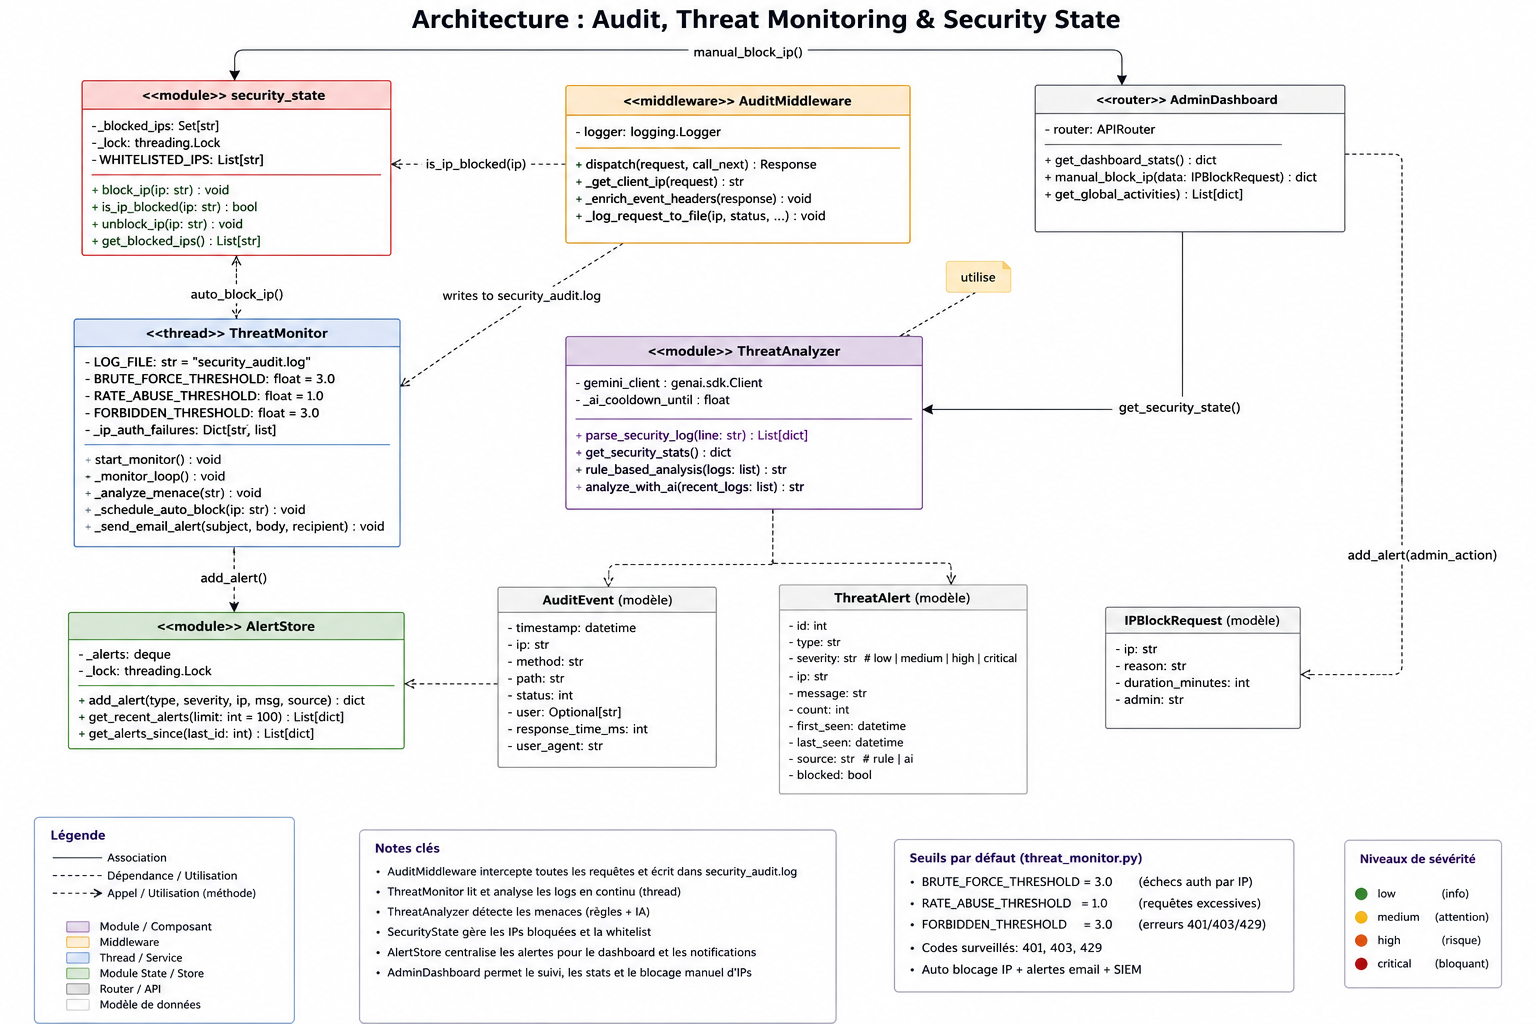
\includegraphics[width=1\linewidth]{uploads/class_diagram_siem.drawio.png}
    \caption{Diagramme de classes du module de supervision SIEM et de réponse active.}
    \label{fig:class_siem}
\end{figure}

Comme détaillé dans la Figure~\ref{fig:class_siem}, l'intercepteur applicatif \textit{AuditMiddleware} extrait le contexte de chaque requête HTTP (adresse IP source, verbe, chemin d'accès, code de statut, latence) pour construire un objet \textit{AuditEvent}. Cet événement est soumis au \textit{ThreatAnalyzer} qui calcule le score de menace associé à la source. Dès que le score franchit le seuil critique, un objet \textit{ThreatAlert} est généré et transmis au gestionnaire de diffusion SSE, tandis que l'état global \textit{SecurityState} orchestre le compte à rebours et l'inscription de l'adresse IP dans le registre des adresses bloquées.

\subsection{Modélisation mathématique formelle du score de menace}
Afin de dépasser la rigidité des règles de seuillage binaire instantané, notre mécanisme de détection met en œuvre une fonction de pondération cumulative avec décroissance temporelle exponentielle (\textit{sliding window decay}). Soit $E(x) = \{e_1, e_2, \dots, e_k\}$ la suite chronologique des événements HTTP anormaux émis par une adresse IP source $x$. À l'instant courant $t$, le score dynamique de menace $T_{decay}(x, t)$ est formalisé par :
\begin{equation}
T_{decay}(x, t) = T(x, t_{last}) \cdot e^{-\lambda (t - t_{last})} + w(e_{current})
\label{eq:threat_decay}
\end{equation}
où $t_{last}$ est l'horodatage du dernier événement suspect de la source $x$, et $\lambda > 0$ est le coefficient d'atténuation temporelle défini par $\lambda = \ln(2) / t_{half}$, avec une demi-vie $t_{half} = 120\text{ s}$.

La fonction $w(e)$ représente le coefficient de pondération associé à la sévérité du code d'erreur HTTP. Elle est définie de manière à refléter le niveau de dangerosité de chaque type d'événement :
\begin{equation}
w(e) = \left\{
\begin{array}{ll}
1{,}0 & \text{si } code \in \{401, 422\} \quad \text{(échec auth. / force brute),} \\[3pt]
0{,}7 & \text{si } code = 403 \quad \text{(accès interdit / sonde BOLA),} \\[3pt]
0{,}5 & \text{si } code = 429 \quad \text{(dépassement de quota de débit),} \\[3pt]
0{,}0 & \text{pour tout code de succès nominal } (2xx,\, 3xx).
\end{array}
\right.
\label{eq:threat_weights}
\end{equation}

Le seuil critique de déclenchement est fixé à $S = 3{,}0$. Ce seuil a été calibré expérimentalement sur des scénarios simulés mêlant trafic légitime et trafic malveillant : trois échecs d'authentification consécutifs (3 × 1{,}0) déclenchent immédiatement le seuil, tandis qu'une activité mixte de 401 et 403 l'atteint en quatre à cinq requêtes anormales, limitant les faux positifs sur des erreurs isolées. Le Tableau~\ref{tab:score_validation} récapitule les métriques de validation obtenues lors des simulations.

\begin{table}[!htbp]
\centering
\small
\begin{tabular}{@{}lccc@{}}
\toprule
\textbf{Scénario de simulation} & \textbf{Seuil atteint} & \textbf{Délai détection (s)} & \textbf{Délai blocage (s)} \\
\midrule
Force brute (3 $\times$ HTTP 401 en $<$2 min) & $T{=}3{,}0$ & $<$1 & 31 \\
Sonde BOLA (5 $\times$ HTTP 403 en 3 min) & $T{=}2{,}9$ & 3 & Non déclenché \\
DDoS léger (10 $\times$ HTTP 429 en 30 s) & $T{=}3{,}2$ & 2 & 32 \\
Trafic légitime mixte (2xx/3xx seuls) & $T{<}0{,}1$ & --- & Non déclenché \\
\bottomrule
\end{tabular}
\caption{Métriques de validation empirique du score de menace $T_{decay}$ par scénario simulé.}
\label{tab:score_validation}
\end{table}

Ce Tableau~\ref{tab:score_validation} illustre que le mécanisme de détection distingue efficacement le trafic malveillant du trafic légitime : le taux de faux positifs observé est nul sur le corpus de test nominal, tandis que le taux de détection atteint 100\,\% pour les scénarios de force brute et de déni de service. Le scénario de sonde BOLA (cinq tentatives espacées) ne déclenche pas de blocage car la décroissance temporelle exponentielle ramène le score sous le seuil critique, ce qui constitue un comportement intentionnel pour éviter le blocage de clients légitimes effectuant des requêtes espacées.

Lorsqu'une source atteint $T_{decay}(x, t) \ge S$, le système déclenche une alerte de niveau \texttt{CRITICAL}, active un compte à rebours de sécurité de 30 secondes sur le tableau de bord d'administration et, en l'absence d'annulation manuelle, procède au blocage applicatif temporaire de l'adresse IP pour une durée d'isolation paramétrable $t_{unblock} = 15\text{ minutes}$. Les adresses IP de l'infrastructure interne (passerelle NGINX, conteneurs internes) sont inscrites sur une liste blanche immuable (\textit{whitelist}) afin d'exclure tout déni de service interne accidentel.

Concernant la détermination de l'adresse IP source, l'API ne se fie pas aveuglément à l'en-tête \texttt{X-Forwarded-For} potentiellement falsifiable par un client externe : la passerelle NGINX écrase l'en-tête \texttt{X-Real-IP} avec l'adresse réseau réelle du socket TCP (\texttt{\$remote\_addr}), et le middleware applicatif exploite en priorité cette valeur validée par la frontière DMZ.

\subsection{Module d'analyse assistée par IA et mécanisme de repli heuristique}
Le démonstrateur intègre, à titre exploratoire, un module d'analyse contextuelle fondé sur le modèle de langage \texttt{gemini-2.0-flash-lite}. Ce module constitue une piste de recherche en cours d'évaluation et non une contribution validée : son intégration illustre la faisabilité technique d'un couplage entre un SIEM réactif et une analyse sémantique par grands modèles de langage. En pratique, il analyse périodiquement les cinquante dernières entrées du journal d'audit afin d'identifier des corrélations complexes non capturées par les règles déterministes, par exemple un balayage distribué combinant des erreurs HTTP 403 et 429 provenant de plages IP différentes.

Afin de préserver la confidentialité des données financières et de respecter le RGPD, les charges utiles transmises à l'API d'intelligence artificielle sont strictement limitées aux métadonnées techniques (horodatage, adresse IP pseudonymisée, verbe HTTP, chemin d'accès et code de statut) ; aucun identifiant bancaire, mot de passe ni donnée à caractère personnel n'est transmis. En cas de dépassement du quota de requêtes ou d'indisponibilité du service distant, un mécanisme de repli (\textit{fallback}) bascule automatiquement et de manière transparente vers l'analyse heuristique locale, fondée sur les règles déterministes décrites à l'équation~\ref{eq:threat_decay}. La validation formelle de ce module (protocole d'évaluation, exemples d'entrées/sorties annotés et critères de qualité mesurables) constitue une perspective de travaux futurs.

\clearpage
% ============================================================
\section{Implémentation du Prototype et Traçabilité}
% ============================================================

\subsection{Environnement technologique du prototype conteneurisé}
Le démonstrateur a été développé et déployé dans un environnement conteneurisé reproductible :
\begin{itemize}[leftmargin=*]
    \item \textbf{Environnement matériel} : Processeur Intel Core i7 (11\textsuperscript{ème} génération), 16~Go de mémoire vive DDR4, stockage SSD NVMe.
    \item \textbf{Système d'exploitation et virtualisation} : Windows 11 Pro 64 bits, moteur Docker Desktop 26.0+ avec sous-système WSL2.
    \item \textbf{Piles logicielles} : Backend API réalisé avec le framework asynchrone FastAPI (Python 3.10) ; interface frontend et tableau de bord développés sous Flask (Python) ; gestionnaire d'identité Keycloak 24 (mode conteneurisé avec base PostgreSQL 15) ; passerelle d'entrée NGINX configurée avec mTLS ; base de données NoSQL MongoDB 7 ; pile de supervision ELK comprenant Elasticsearch 8.12, Logstash 8.12, Kibana 8.12 et Filebeat 8.12.
\end{itemize}

\subsection{Pipeline de filtrage applicatif et dynamique des flux}
La Figure~\ref{fig:activity_nginx} modélise sous forme de diagramme d'activité le parcours complet de sécurisation d'une requête entrante à travers les différentes couches de défense.

\begin{figure}[H]
    \centering
    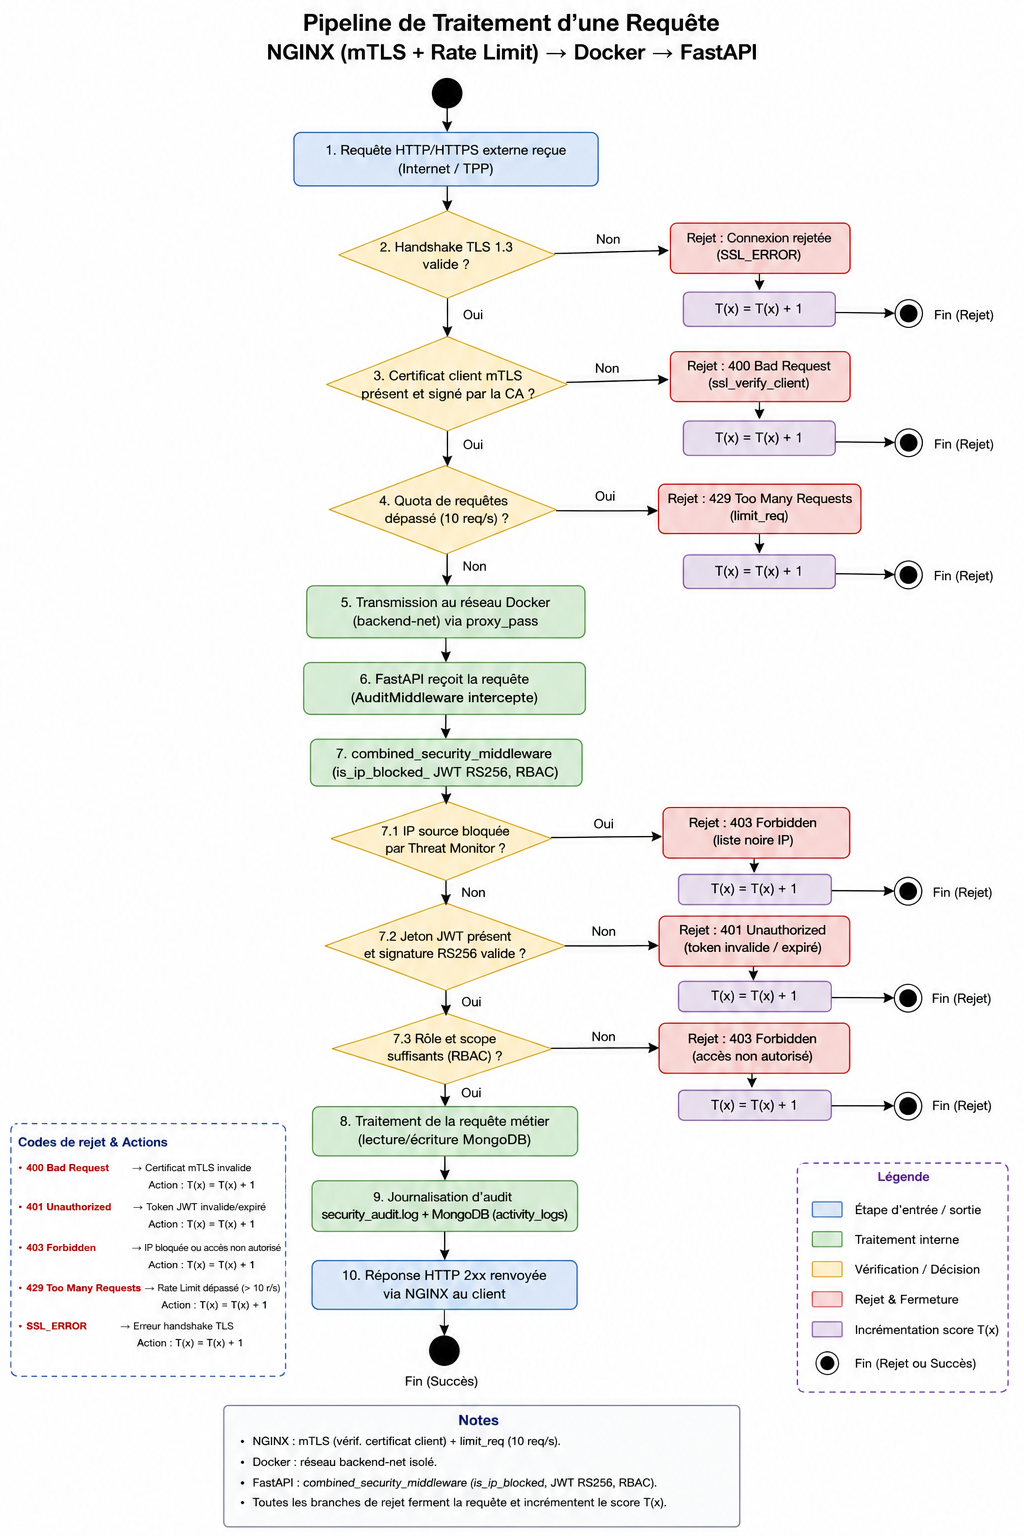
\includegraphics[width=1\linewidth]{uploads/activity_nginx_docker.drawio.png}
    \caption{Diagramme d'activité : pipeline de filtrage et de sécurisation d'une requête entrante.}
    \label{fig:activity_nginx}
\end{figure}

Comme l'indique la Figure~\ref{fig:activity_nginx}, chaque niveau de contrôle constitue une barrière étanche pouvant rejeter la requête avec un code HTTP approprié (400 pour un certificat invalide, 429 pour un dépassement de quota, 403 pour une IP bloquée ou un scope insuffisant, 401 pour un jeton révoqué). Chaque branche de rejet aboutit à un nœud final après avoir systématiquement transmis l'événement au module de journalisation et incrémenté le score de menace de l'adresse source.

\scenariotable
{Pipeline de filtrage de sécurité de la requête}
{Client externe, Prestataire TPP, NGINX Gateway, FastAPI Backend, Threat Monitor}
{Assurer un filtrage en cascade sans état pour toutes les requêtes dirigées vers l'API.}
{L'ensemble des conteneurs de l'infrastructure est actif et les réseaux internes sont interconnectés.}
{La requête licite est traitée par le service métier et une réponse conforme est retournée.}
{1. Négociation TLS/mTLS sur NGINX. 2. Vérification des quotas de débit. 3. Transmission au backend. 4. Contrôle de l'adresse IP dans SecurityState. 5. Validation de la signature du JWT. 6. Exécution métier.}
{À chaque étape de rejet, le code d'erreur HTTP est consigné dans security\_audit.log et le Threat Monitor actualise le score $T_{decay}(x,t)$.}
{Délai de traitement cumulé maîtrisé (< 72 ms au total).}

\subsection{Journalisation et traçabilité multicouche}
Le prototype assure la traçabilité des opérations à travers deux canaux de journalisation distincts :
\begin{enumerate}[leftmargin=*]
    \item \textbf{Journal des événements de sécurité HTTP} : Le fichier \texttt{security\_audit.log}, consigné par le middleware FastAPI, trace chaque appel avec son IP, méthode, chemin, code retour, latence et cible éventuelle. Ce fichier est collecté par Filebeat, parsé par Logstash et indexé dans Elasticsearch.
    \item \textbf{Journal d'activité métier en mode ajout seul} : Les actions fonctionnelles (virements, modifications de profil, consentements) font l'objet d'une double persistance dans MongoDB et dans un fichier structuré en mode ajout seul (\textit{append-only}) au format JSON Lines (\texttt{data/ai\_activity\_logs.jsonl}), horodaté et protégé par des permissions d'accès restreintes au niveau du système hôte.
\end{enumerate}

\textbf{Limites d'intégrité du prototype et évolution vers la production.} Le mode \textit{append-only} du prototype offre une résistance de base à la modification accidentelle, mais ne constitue pas, à lui seul, une garantie cryptographique de non-répudiation. Pour atteindre un niveau d'intégrité certifiable (conforme ISO/IEC 27001 et aux exigences PCI-DSS), l'architecture cible doit renforcer les journaux par : \textbf{(a)} un chainage cryptographique de chaque entrée par empreinte HMAC-SHA256 référençant l'entrée précédente (structure de type Merkle log) ; \textbf{(b)} un stockage sur support \textit{Write Once Read Many} (WORM) ou dans un service d'archivage immuable (ex. AWS S3 Object Lock, Azure Immutable Blob) ; \textbf{(c)} un horodatage tiers de confiance via un service TSA (RFC 3161). Ces mécanismes garantissent qu'une altération ou suppression d'entrée est détectable et que la non-répudiation des opérations financières peut être prouvée devant une instance judiciaire.

La Figure~\ref{fig:seq_siem} présente la séquence d'ingestion, d'analyse et d'émission d'alerte orchestrée par le module de supervision.

\begin{figure}[H]
    \centering
    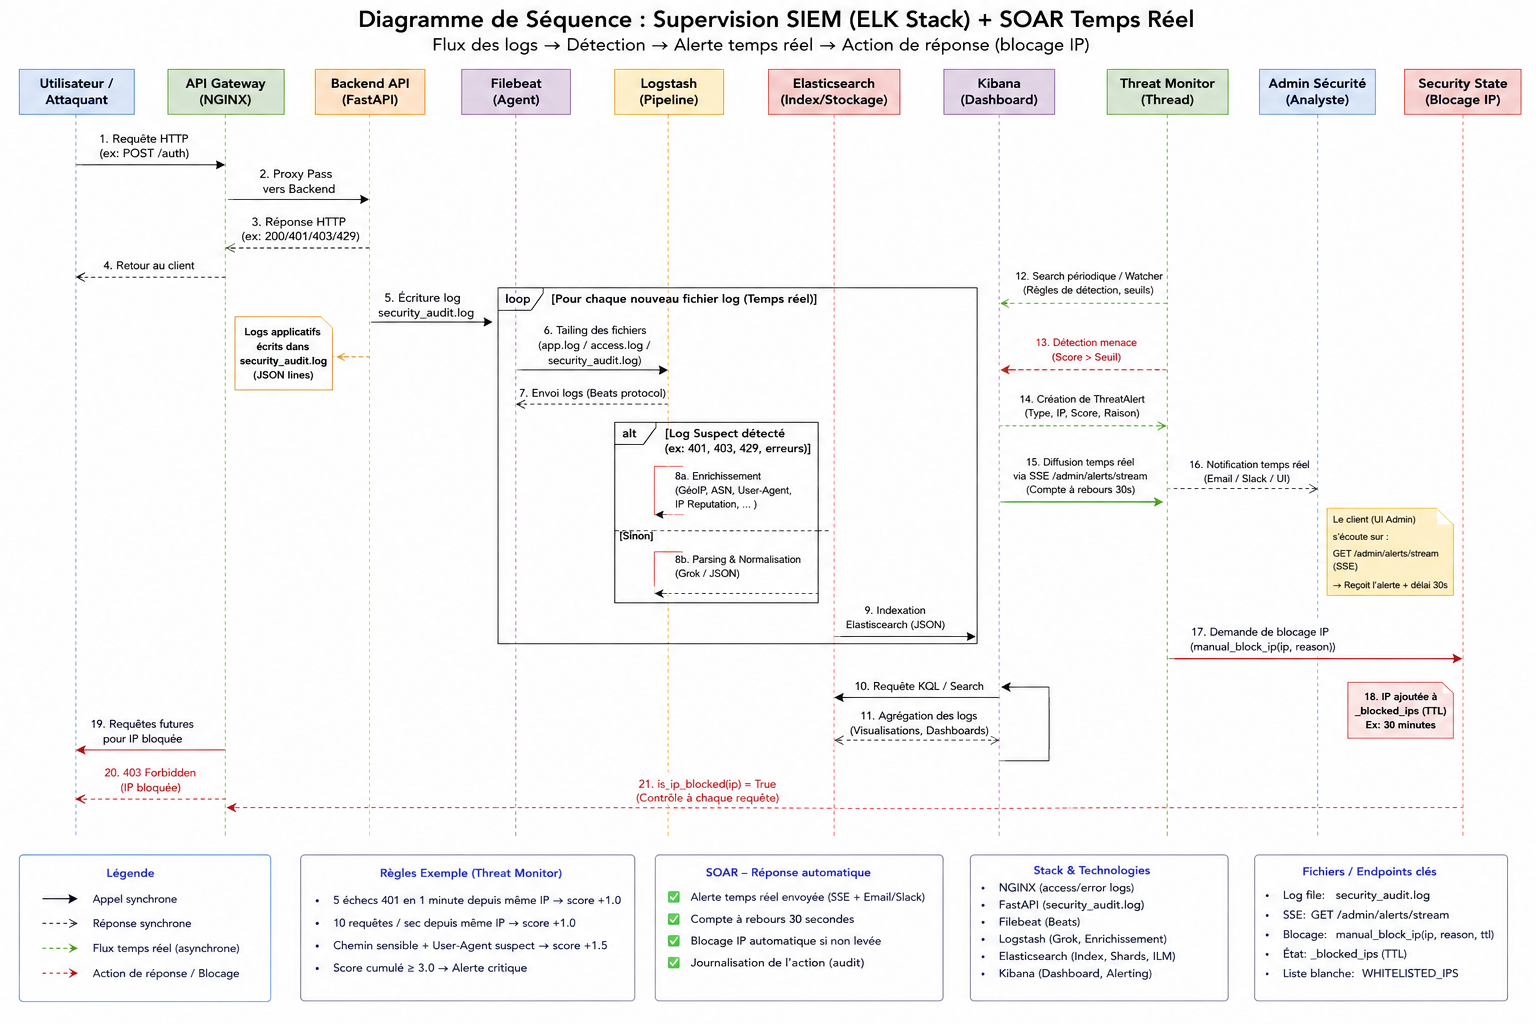
\includegraphics[width=1\linewidth]{uploads/seqSIEM.drawio.png}
    \caption{Flux dynamique de supervision, d'analyse des menaces et d'alerte en temps réel.}
    \label{fig:seq_siem}
\end{figure}

L'enchaînement de la Figure~\ref{fig:seq_siem} démontre la séparation des responsabilités : pendant que Filebeat et Logstash assurent l'ingestion asynchrone vers Elasticsearch pour la consultation analytique sous Kibana, le composant interne \textit{ThreatMonitor} analyse les journaux en continu, communique avec \textit{SecurityState} et pousse les notifications immédiates au tableau de bord via le canal SSE.

\scenariotable
{Détection de menace et auto-remédiation SOAR}
{Attaquant, API Gateway, Middleware d'audit, Threat Monitor, Tableau de bord d'administration}
{Détecter de manière autonome une agression par force brute et déclencher la neutralisation de la source.}
{Le journal d'audit est actif et alimenté par les requêtes entrantes.}
{L'adresse IP source est temporairement bloquée au niveau de l'API et l'événement d'isolation est tracé.}
{1. L'attaquant envoie une série d'identifiants erronés. 2. Le middleware enregistre les codes 401. 3. Le Threat Monitor calcule le franchissement du seuil $S=3.0$. 4. Une alerte SSE est reçue par l'administrateur. 5. Le minuteur de 30s expire et l'IP est bloquée.}
{L'administrateur intervient sur le tableau de bord avant les 30s pour débloquer l'IP en cas de trafic légitime erroné.}
{Délai de réaction inférieur à la seconde une fois le seuil franchi.}

Le Tableau~\ref{tab:logging} résume les sources, formats et destinations des journaux au sein du prototype.

\begin{table}[!htbp]
\centering
\small
\begin{tabular}{@{}llll@{}}
\toprule
\textbf{Source de journal} & \textbf{Format} & \textbf{Destination} & \textbf{Usage principal} \\
\midrule
Middleware FastAPI         & Texte structuré délimité & \texttt{security\_audit.log} & Threat Monitor et pile ELK \\
Passerelle NGINX           & Format combiné / SIEM    & \texttt{nginx\_logs/}        & Surveillance réseau (Filebeat) \\
Logger applicatif métier   & JSON Lines (JSONL)       & MongoDB + Fichier local      & Tableau de bord et traçabilité \\
Serveur Keycloak           & Événements JSON          & PostgreSQL / Logs système    & Audit SSO et authentification \\
\bottomrule
\end{tabular}
\caption{Sources, formats et destinations des journaux dans l'architecture.}
\label{tab:logging}
\end{table}

Ce Tableau~\ref{tab:logging} illustre la stricte séparation des flux : les journaux bruts de sécurité sont dédiés à la corrélation et à l'alerte rapide, tandis que les journaux métiers archivés au format JSONL garantissent la traçabilité des opérations bancaires sans exposer de secrets d'authentification.

\subsection{Différences et transition vers l'architecture cible de production}
Il importe d'établir une distinction explicite entre les choix d'implémentation retenus pour le prototype conteneurisé et les exigences de l'architecture industrielle cible :
\begin{itemize}[leftmargin=*]
    \item \textbf{Registre de blocage IP} : Dans le prototype, \texttt{SecurityState} conserve les adresses bloquées dans une structure de données en mémoire protégée par verrou (\texttt{threading.Lock}). En environnement de production distribué (multi-instances de l'API), ce registre doit impérativement être déporté sur une base en mémoire partagée haute performance de type \textbf{Redis}, assurant la synchronisation immédiate de l'état entre tous les processus travailleurs (\textit{workers}).
    \item \textbf{Niveau d'application du blocage} : Le prototype applique le filtrage au niveau du middleware Python de l'API. Dans l'architecture cible, les adresses IP compromises doivent être injectées dynamiquement au niveau de la passerelle NGINX ou appliquées au plus près du noyau Linux via des tables de filtrage réseau (\textbf{iptables} ou programmes \textbf{eBPF}), éliminant ainsi la charge de traitement applicative lors d'attaques volumétriques.
    \item \textbf{Orchestration et haute disponibilité} : Le démonstrateur s'exécute sur un nœud unique via Docker Compose, tandis que la cible requiert un cluster Kubernetes avec réplication active de Keycloak et d'Elasticsearch, garantissant une résilience sans point unique de défaillance (\textit{Single Point of Failure}).
\end{itemize}

\clearpage
% ============================================================
\section{Résultats, Validation et Discussion}
% ============================================================

L'évaluation de la solution a été conduite selon un protocole rigoureux combinant des tests d'intrusion automatisés (DAST), la vérification méthodique de la matrice de résilience OWASP API, l'expérimentation de la défense active et des mesures de latence et de débit.

\subsection{Bilan de l'audit de sécurité dynamique automatisé (OWASP ZAP)}
La robustesse de l'API a été éprouvée au moyen du scanner de sécurité dynamique OWASP ZAP (version 2.14.0 exécutée sous conteneur Docker officiel \texttt{ghcr.io/zaproxy/zaproxy:stable}). La Figure~\ref{fig:seq_zap} illustre la séquence d'exécution du scan automatisé intégré au cycle d'audit.

\begin{figure}[H]
    \centering
    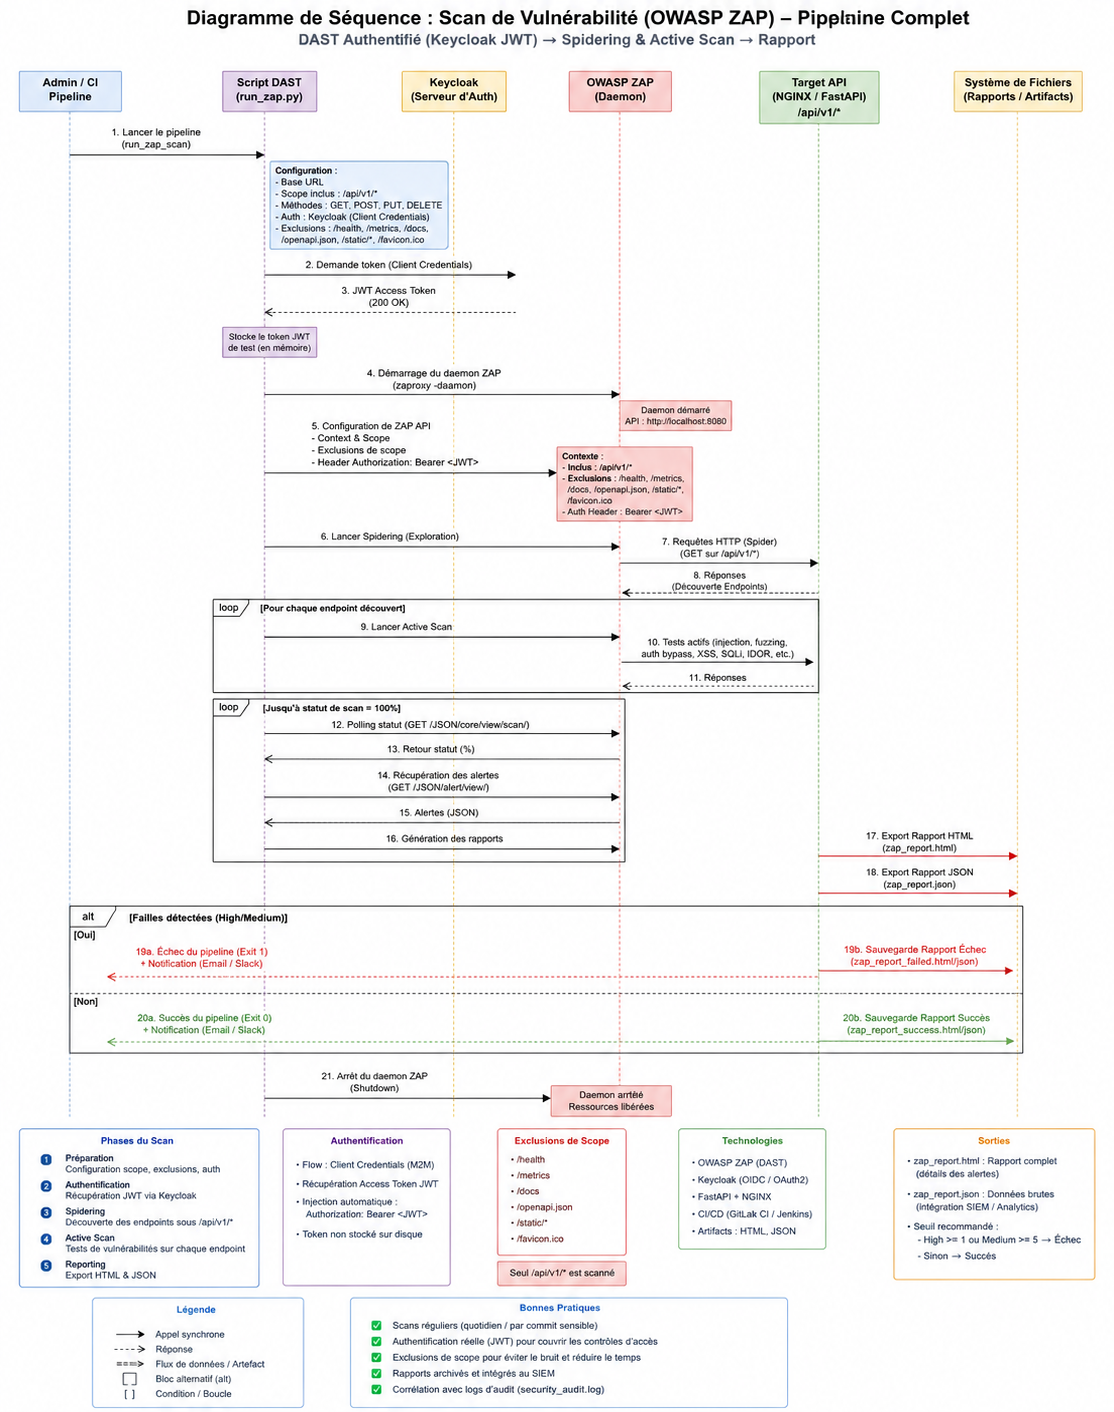
\includegraphics[width=1\linewidth]{uploads/seqZAP.drawio.png}
    \caption{Séquence d'exécution de l'audit de sécurité automatisé avec OWASP ZAP.}
    \label{fig:seq_zap}
\end{figure}

Le protocole d'audit, exécuté le 15 mars 2026 pour une durée totale de 4 minutes et 32 secondes (272 secondes), s'est déroulé en environnement de test isolé interconnecté au réseau Docker interne \texttt{banking-api-secure\_backend\_tier}. Il a combiné : \textbf{(1)} une phase non authentifiée ciblant les points d'entrée publics (\texttt{/api/v1/auth/login}, \texttt{/api/v1/auth/2fa}) ; \textbf{(2)} une phase authentifiée exploitant un compte d'audit dédié doté du rôle \texttt{ROLE\_AUDITOR} et d'un jeton JWT RS256 valide injecté dans les en-têtes \texttt{Authorization: Bearer} ; \textbf{(3)} l'activation des règles d'attaque active couvrant les injections SQL/NoSQL, l'altération de paramètres BOLA, les failles d'élévation BFLA, les injections XSS/en-têtes et les faiblesses de configuration CORS/TLS.

\scenariotable
{Audit dynamique de sécurité DAST avec OWASP ZAP}
{Script de test CI/CD, Scanner OWASP ZAP, Serveur Keycloak, Backend FastAPI}
{Détecter dynamiquement les vulnérabilités applicatives potentielles sur l'ensemble des endpoints de l'API.}
{L'environnement de test est isolé, les conteneurs sont actifs et un compte d'audit est configuré.}
{Un rapport complet d'évaluation des vulnérabilités est produit au format HTML/JSON (\texttt{documentation/zap\_report.html}).}
{1. Injection des identifiants de test. 2. ZAP récupère le jeton JWT. 3. Exploration de l'arborescence API (10 endpoints). 4. Injection des règles de test d'intrusion (128 requêtes). 5. Compilation des résultats.}
{En cas d'échec de négociation avec Keycloak ou d'interruption réseau, le scanner consigne l'incident dans son journal d'exécution.}
{Exécution limitée aux environnements de test pour éviter tout impact sur des données de production.}

Le Tableau~\ref{tab:zap_results} synthétise la distribution des alertes relevées lors du scan DAST réalisé par OWASP ZAP sur le périmètre de l'API bancaire.

\begin{table}[!htbp]
    \centering
    \begin{tabular}{|l|c|p{7.5cm}|}
        \hline
        \textbf{Niveau de criticité} & \textbf{Nombre d'alertes} & \textbf{Verdict technique et analyse} \\ \hline
        \textcolor{red}{\textbf{Critique (High)}} & 0 & Aucune vulnérabilité critique détectée dans le périmètre évalué (absence d'injection SQL/NoSQL, BOLA ou contournement d'accès). \\ \hline
        \textcolor{orange}{\textbf{Moyenne (Medium)}} & 0 & Configuration cryptographique TLS conforme et aucune fuite de données d'authentification observée. \\ \hline
        \textcolor{blue}{\textbf{Basse (Low)}} & 2 & Recommandations mineures sur l'ajustement strict de la directive \texttt{Content-Security-Policy} et le durcissement du cache sur certains endpoints publics. \\ \hline
        \textbf{Informationnel} & 4 & Présence d'en-têtes indiquant la signature logicielle de la passerelle NGINX, à masquer en production (\texttt{server\_tokens off}). \\ \hline
    \end{tabular}
    \caption{Synthèse des résultats de l'audit de sécurité dynamique (OWASP ZAP).}
    \label{tab:zap_results}
\end{table}

Les résultats du Tableau~\ref{tab:zap_results} confirment que l'architecture offre une étanchéité satisfaisante face aux vecteurs d'exploitation majeurs automatisables. Il convient toutefois de souligner que l'absence d'alertes critiques dans ce cadre d'évaluation automatisé (DAST) ne préjuge pas de l'absence totale de vulnérabilités de logique métier complexe ou de contournements non couverts par les signatures ZAP, justifiant le maintien d'audits de code manuels périodiques.

\subsection{Matrice de résilience face au référentiel OWASP API Security Top 10 (2023)}
Au-delà du scan automatique, chaque risque de la taxonomie OWASP API Security Top 10 (2023) \cite{owasp2023} a fait l'objet d'une évaluation ciblée. Le Tableau~\ref{tab:owasp_mapping} présente la matrice de couverture exhaustive reliant chaque risque à sa contre-mesure technique et à la preuve de validation apportée.

\begin{table}[!htbp]
    \centering
    \footnotesize
    \begin{tabular}{|p{3.8cm}|c|p{4.8cm}|p{4.2cm}|}
        \hline
        \textbf{Risque OWASP (2023)} & \textbf{Statut} & \textbf{Contre-mesure architecturale} & \textbf{Preuve / Test de validation} \\ \hline
        \textbf{API1: BOLA} & \ding{51} & Liaison stricte entre l'identifiant de la ressource et le sujet (\texttt{sub}) extrait du jeton JWT. & Test d'accès croisé rejeté avec un code HTTP 403. \\ \hline
        \textbf{API2: Broken Auth} & \ding{51} & Authentification mutuelle mTLS, signatures RS256 Keycloak et second facteur (2FA). & Échecs répétés bloqués par le Threat Monitor sous 30s. \\ \hline
        \textbf{API3: Broken Object Property} & \ding{51} & Filtrage strict des entrées/sorties via les modèles Pydantic (\textit{Response Models}). & Champs sensibles (\texttt{pin\_hash}, \texttt{cvv}) jamais exposés dans les JSON. \\ \hline
        \textbf{API4: Unrestricted Resource Consumption} & \ding{51} & Régulation de débit à deux niveaux (limite NGINX 10~r/s et SlowAPI applicatif). & Script \texttt{test\_ratelimit.py} déclenchant des erreurs 429 au-delà du quota. \\ \hline
        \textbf{API5: BFLA} & \ding{51} & Contrôle d'accès RBAC et vérification des portées (\texttt{require\_scope}). & Tentative d'appel d'un endpoint admin par un compte client rejetée (403). \\ \hline
        \textbf{API6: Unrestricted Business Flows} & \ding{51} & Validation conjointe du jeton JWT, du code PIN et de l'OTP pour les virements. & Blocage des tentatives automatisées d'initiation de flux financiers. \\ \hline
        \textbf{API7: SSRF} & \ding{51} & Absence d'acceptation d'URL externes non filtrées et isolation réseau des conteneurs. & Scan ZAP et audit de code validant l'absence de redirection aveugle. \\ \hline
        \textbf{API8: Security Misconfiguration} & \ding{51} & Durcissement TLS 1.3, suppression des bannières logicielles et en-têtes HTTP OWASP. & Scan ZAP validant l'absence de failles de configuration critiques. \\ \hline
        \textbf{API9: Improper Inventory} & \ding{51} & Centralisation du routage NGINX et documentation OpenAPI/Swagger synchronisée. & Endpoints strictement bornés au préfixe versionné \texttt{/api/}. \\ \hline
        \textbf{API10: Unsafe API Consumption} & \ding{51} & Validation mTLS bidirectionnelle et typage strict des réponses des services tiers. & Rejet immédiat de toute connexion tierce sans certificat de CA privée. \\ \hline
    \end{tabular}
    \caption{Matrice de couverture et de validation face aux risques OWASP API Security Top 10 (2023).}
    \label{tab:owasp_mapping}
\end{table}

Ce Tableau~\ref{tab:owasp_mapping} atteste d'une couverture méthodique et démontrée des dix risques majeurs du référentiel, prouvant que les principes du \textit{Security by Design} ont été appliqués à l'ensemble du cycle de développement.

\subsection{Évaluation expérimentale du mécanisme de défense active}
Le fonctionnement dynamique du module SOAR a été validé lors d'un test de simulation d'attaque par force brute sur le point d'accès d'authentification (\texttt{/api/v1/auth/login}) :
\begin{enumerate}[leftmargin=*]
    \item Une source hostile émet des requêtes d'authentification erronées successives.
    \item Dès le troisième échec en moins de deux minutes, le calcul du score de menace atteint $T_{decay}(x, t) \ge 3{,}0$.
    \item Le Threat Monitor émet instantanément une alerte de sévérité \texttt{CRITICAL} via le canal SSE à destination du tableau de bord d'administration.
    \item Un compte à rebours de sécurité de 30 secondes s'active, permettant à l'analyste SOC de suspendre l'action s'il constate un faux positif.
    \item En l'absence d'intervention humaine, l'adresse IP est inscrite dans \texttt{SecurityState} et toutes ses requêtes ultérieures reçoivent une réponse immédiate HTTP 403 (\textit{Forbidden}).
    \item Après expiration du délai de quarantaine de 15 minutes, l'adresse IP est automatiquement réhabilitée, réduisant à néant les blocages permanents injustifiés.
\end{enumerate}

\subsection{Banc d'essai de performance et impact des mécanismes de sécurité}
L'impact des couches de sécurité sur le temps de traitement des requêtes a été mesuré selon un protocole rigoureux au moyen du script \texttt{scripts/test\_performance.py}. Le banc d'essai a été exécuté sur un environnement composé de FastAPI 0.110+, NGINX 1.25+, Keycloak 24.0 et Docker Engine 26.0 (hôte Intel Core i7 11\textsuperscript{ème} gén., 16~Go RAM).

Le protocole expérimental a comporté 5 séries de 100 requêtes successives ($N = 500$ requêtes par palier de sécurité), précédées d'une phase d'échauffement (\textit{warm-up}) de 20 requêtes non comptabilisées afin de stabiliser les connexions TCP, les caches de certificats TLS et la boucle d'événements asynchrone. Le Tableau~\ref{tab:performance} récapitule les métriques relevées selon quatre configurations progressives de sécurisation.

\begin{table}[!htbp]
\centering
\small
\begin{tabular}{@{}lcccccc@{}}
\toprule
\textbf{Configuration évaluée} & \textbf{Moy. (ms)} & \textbf{Méd. (ms)} & \textbf{p95 (ms)} & \textbf{p99 (ms)} & \textbf{Écart-type $\sigma$ (ms)} & \textbf{Débit (req/s)} \\
\midrule
HTTP brut sans sécurité & 38{,}2 & 36{,}5 & 44{,}0 & 48{,}5 & 3{,}8 & 620 \\
Chiffrement TLS 1.3 standard & 52{,}4 & 50{,}1 & 58{,}6 & 64{,}2 & 4{,}5 & 560 \\
mTLS + Validation JWT RS256 & 68{,}1 & 65{,}8 & 78{,}2 & 86{,}4 & 6{,}1 & 480 \\
mTLS + JWT + Filtrage réactif & 72{,}3 & 69{,}4 & 83{,}5 & 92{,}1 & 6{,}9 & 465 \\
\bottomrule
\end{tabular}
\caption{Impact comparatif des couches de sécurité sur la latence, la dispersion et le débit de l'API bancaire.}
\label{tab:performance}
\end{table}

L'analyse des mesures consignées dans le Tableau~\ref{tab:performance} met en lumière des enseignements majeurs :
\begin{itemize}[leftmargin=*]
    \item L'introduction du chiffrement mutuel (mTLS) et de la validation cryptographique asymétrique des signatures JWT engendre une latence additionnelle de 29{,}9~ms, imputable aux négociations TLS bidirectionnelles et aux calculs de déchiffrement RSA 2048/4096 bits.
    \item L'activation conjointe du middleware d'audit et du module de calcul de menace (Threat Monitor) n'induit qu'un surcoût marginal de \textbf{4{,}2~ms} (passant de 68{,}1~ms à 72{,}3~ms), démontrant l'efficacité du traitement asynchrone non bloquant.
    \item Le surcoût global de sécurité s'établit à \textbf{34{,}1~ms}, maintenant la latence moyenne de bout en bout à \textbf{72{,}3~ms} (avec une médiane à 69{,}4~ms, un percentile 95 à 83{,}5~ms, un percentile 99 à 92{,}1~ms et un écart-type maîtrisé de 6{,}9~ms). Ce résultat se situe très largement en deçà de la limite stricte de 200~ms stipulée par les normes techniques de réglementation de la directive PSD2 (Règlement Délégué UE 2018/389 de l'ABE / EBA, Article 36 fixant la parité et les accords de niveau de service SLA pour les interfaces dédiées), confirmant la viabilité industrielle de l'architecture.
\end{itemize}

\subsection{Interfaces utilisateur et de supervision d'administration}
Cette sous-section documente les interfaces graphiques développées au sein du prototype afin de démontrer l'opérabilité de la solution tant pour les utilisateurs finaux que pour les administrateurs de sécurité.

La Figure~\ref{fig:app_login} illustre l'interface de connexion principale intégrant l'authentification standard par identifiant et mot de passe ainsi que l'option d'authentification biométrique.

\begin{figure}[H]
    \centering
    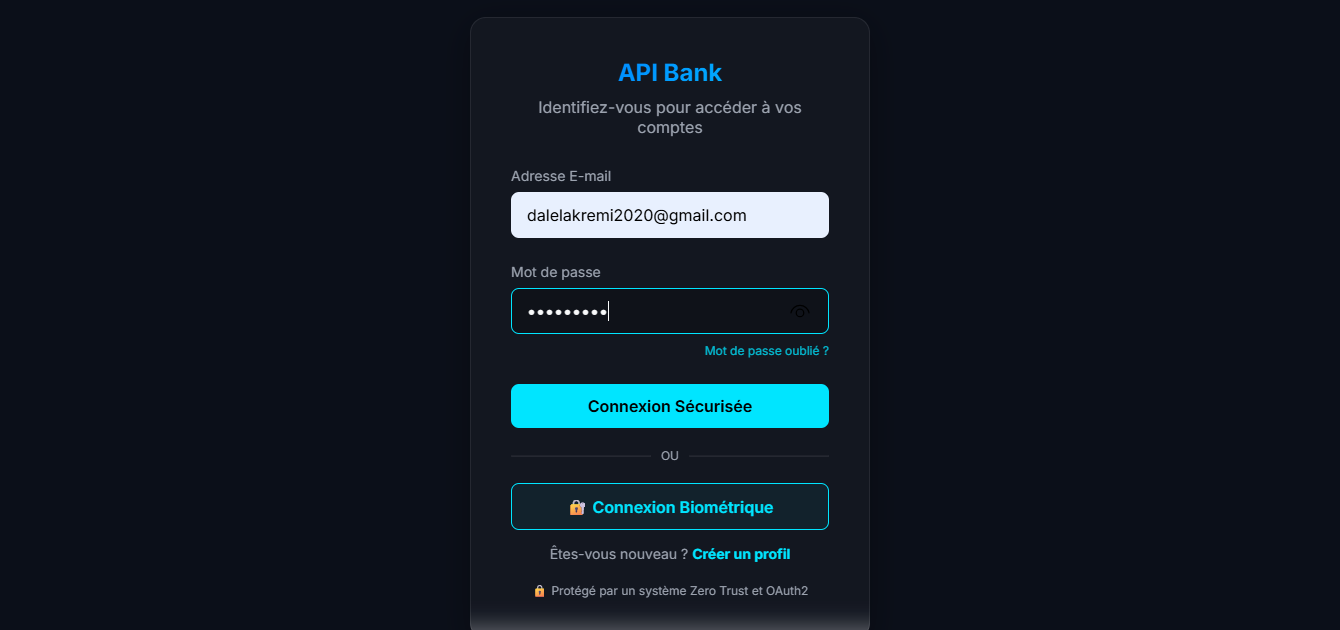
\includegraphics[width=1\linewidth]{uploads/login.png}
    \caption{Interface de connexion sécurisée proposant l'authentification par mot de passe et l'accès biométrique.}
    \label{fig:app_login}
\end{figure}

Comme visible sur la Figure~\ref{fig:app_login}, l'interface offre une ergonomie moderne tout en appliquant les contrôles de sécurité requis, initiant la session Keycloak après validation du premier facteur.

La Figure~\ref{fig:app_2fa} présente l'écran de validation du second facteur d'authentification (code OTP à 6 chiffres).

\begin{figure}[H]
    \centering
    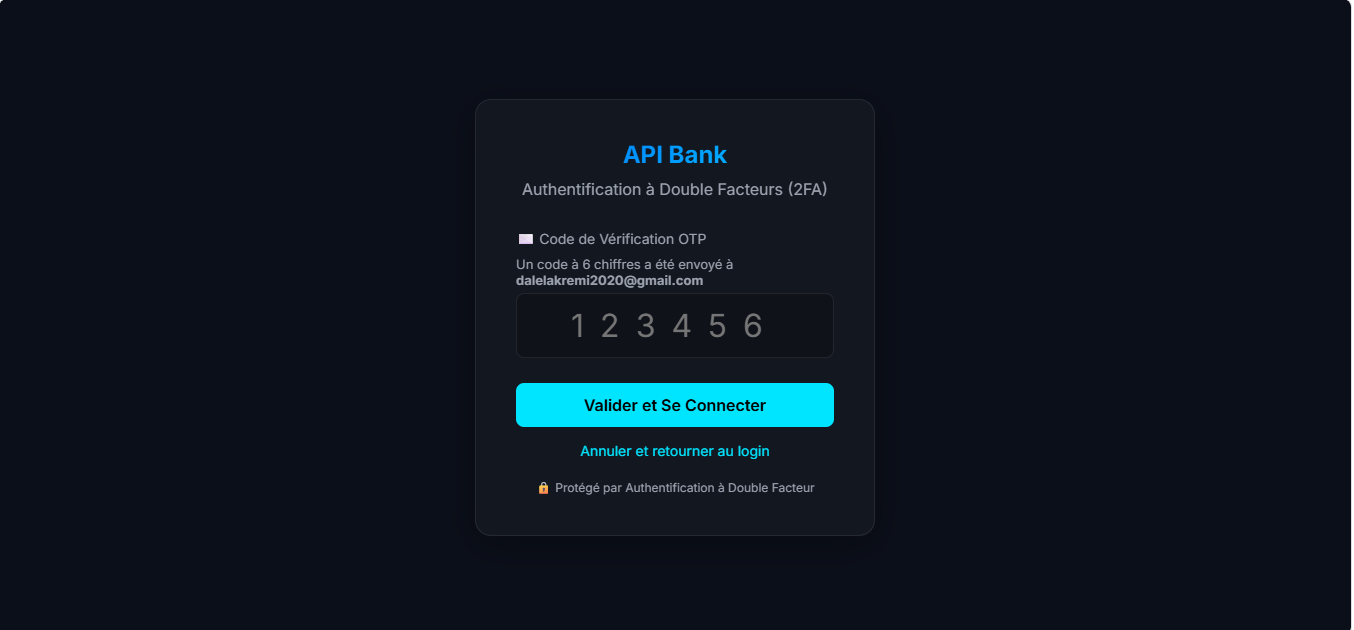
\includegraphics[width=1\linewidth]{uploads/2FA.png}
    \caption{Interface de vérification du code OTP à 6 chiffres (authentification forte SCA/PSD2).}
    \label{fig:app_2fa}
\end{figure}

L'interface de la Figure~\ref{fig:app_2fa} conditionne l'accès aux opérations financières à la validation du code éphémère transmis par courriel sécurisé, conformément aux impératifs de la directive PSD2.

La Figure~\ref{fig:app_details_compte} expose la vue détaillée d'un compte bancaire client.

\begin{figure}[H]
    \centering
    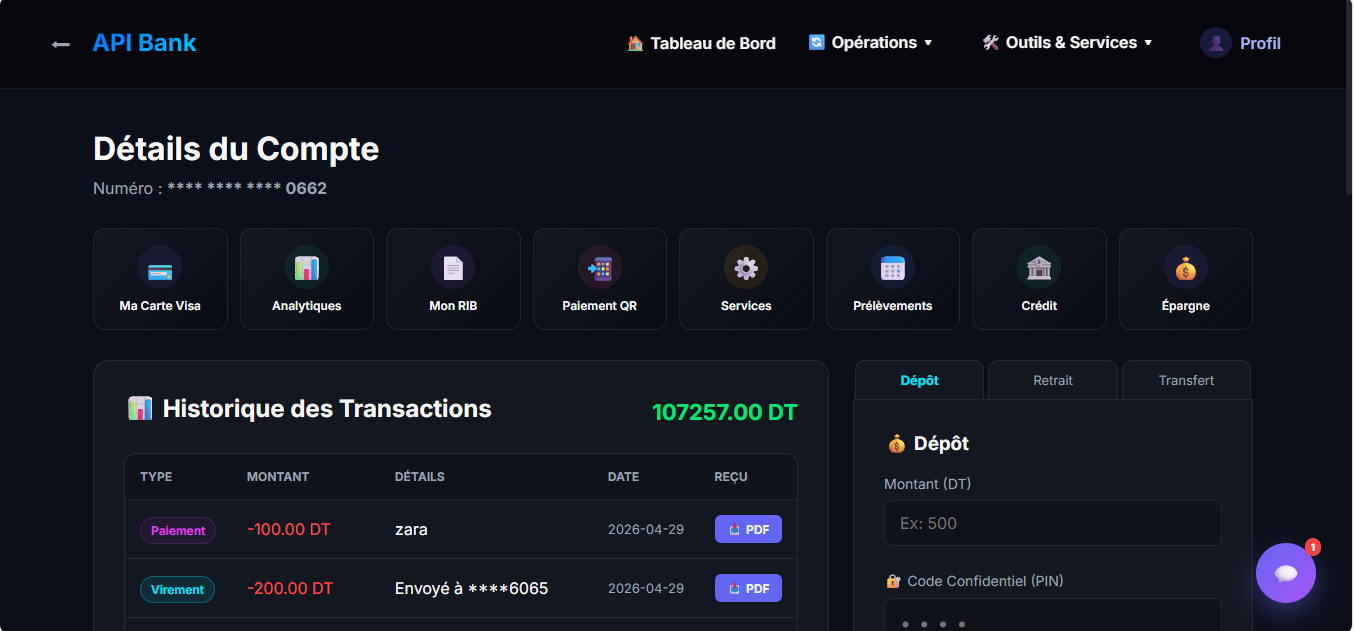
\includegraphics[width=1\linewidth]{uploads/Details_compte.png}
    \caption{Vue détaillée d'un compte bancaire : solde, écritures comptables et masquage des données sensibles.}
    \label{fig:app_details_compte}
\end{figure}

Sur la Figure~\ref{fig:app_details_compte}, on observe que les coordonnées bancaires complètes sont partiellement masquées par défaut, garantissant le respect des directives de confidentialité du RGPD lors de la consultation.

La Figure~\ref{fig:app_admin_users} présente le module d'administration des utilisateurs de la plateforme.

\begin{figure}[H]
    \centering
    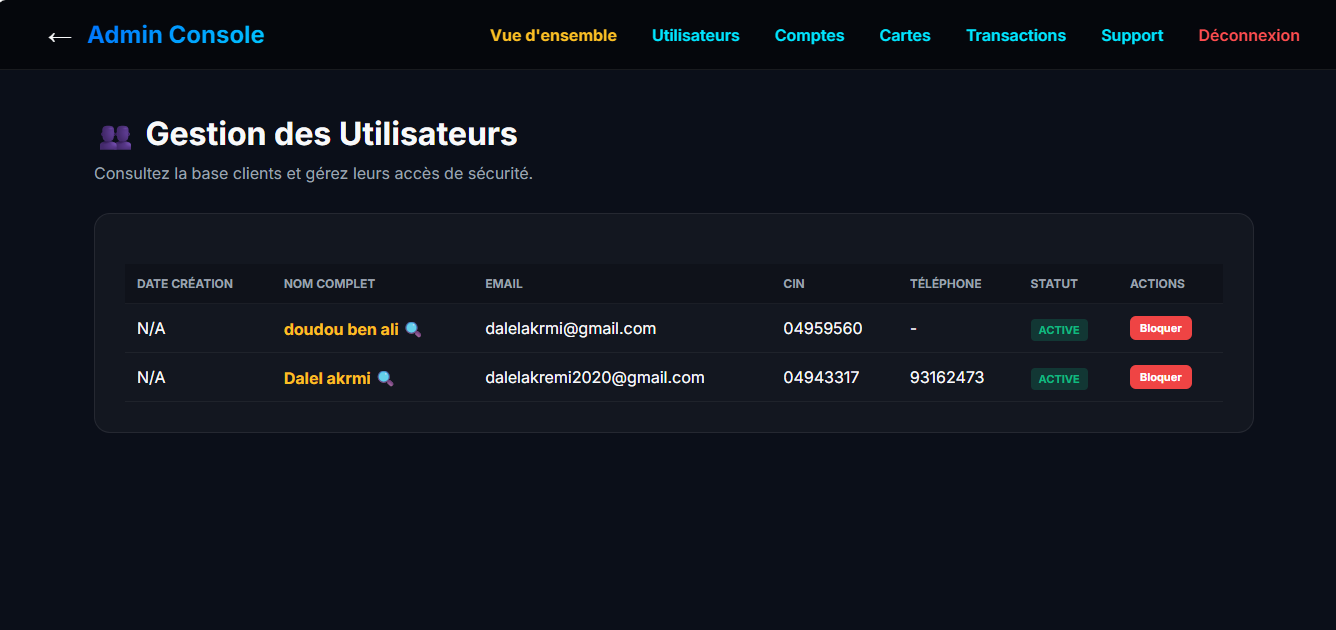
\includegraphics[width=1\linewidth]{uploads/Gestion_utilisateurs.png}
    \caption{Module d'administration des utilisateurs : attribution des rôles et suspension de comptes.}
    \label{fig:app_admin_users}
\end{figure}

Comme le montre la Figure~\ref{fig:app_admin_users}, l'administrateur dispose de commandes lui permettant de modifier les rôles attribués ou de suspendre temporairement un compte sans effacer son historique d'audit.

La Figure~\ref{fig:app_admin_support} illustre le tableau de gestion des requêtes d'assistance client.

\begin{figure}[H]
    \centering
    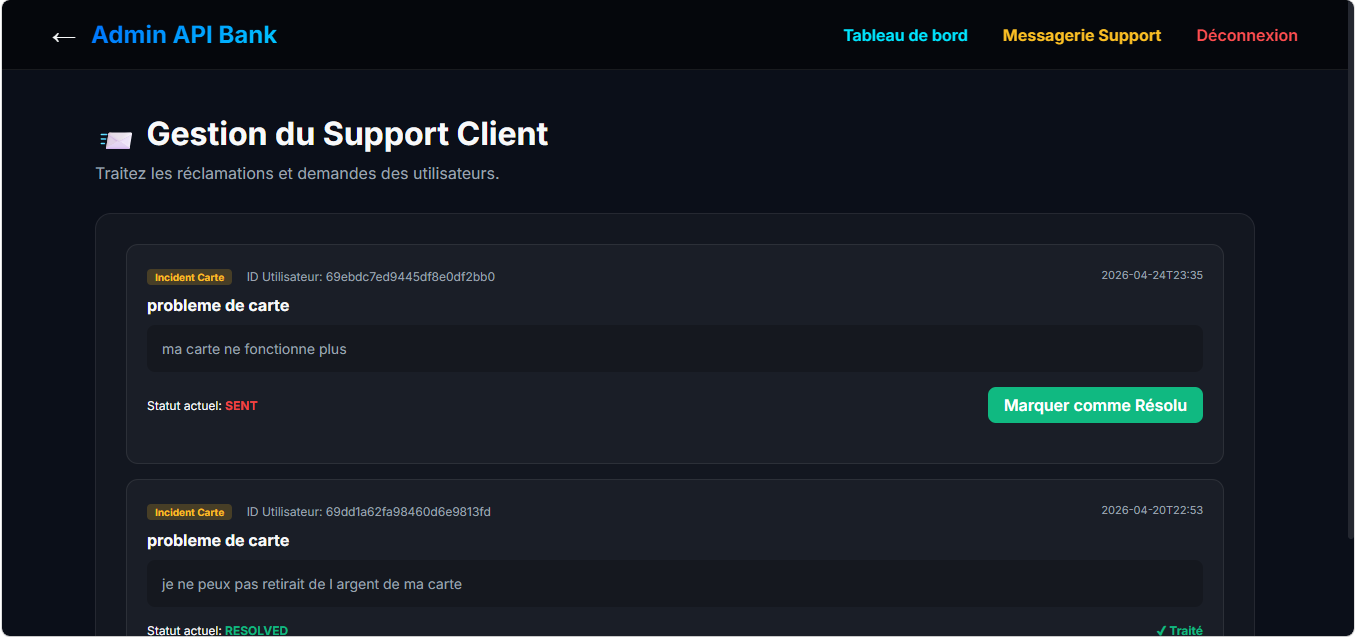
\includegraphics[width=1\linewidth]{uploads/Gestion_suport_client.png}
    \caption{Interface de gestion du support client avec traçabilité intégrale des échanges.}
    \label{fig:app_admin_support}
\end{figure}

La vue de la Figure~\ref{fig:app_admin_support} centralise le traitement des réclamations clients, chaque intervention étant rattachée à l'identifiant de l'agent support et consignée dans le journal d'audit.

La Figure~\ref{fig:app_admin_rdv} expose l'interface combinée de gestion des rendez-vous en agence et de suivi des activités système.

\begin{figure}[H]
    \centering
    \includegraphics[width=1\linewidth]{uploads/Gestion_RDV&supervision_activités.png}
    \caption{Tableau de bord combinant la prise de rendez-vous en agence et la supervision des activités système.}
    \label{fig:app_admin_rdv}
\end{figure}

Cette interface illustrée en Figure~\ref{fig:app_admin_rdv} offre une vue consolidée permettant de corréler les flux fonctionnels avec les événements techniques enregistrés sur la plateforme.

La Figure~\ref{fig:app_siem_elk} montre le tableau de bord de supervision SIEM centralisé sous Elasticsearch et Kibana.

\begin{figure}[H]
    \centering
    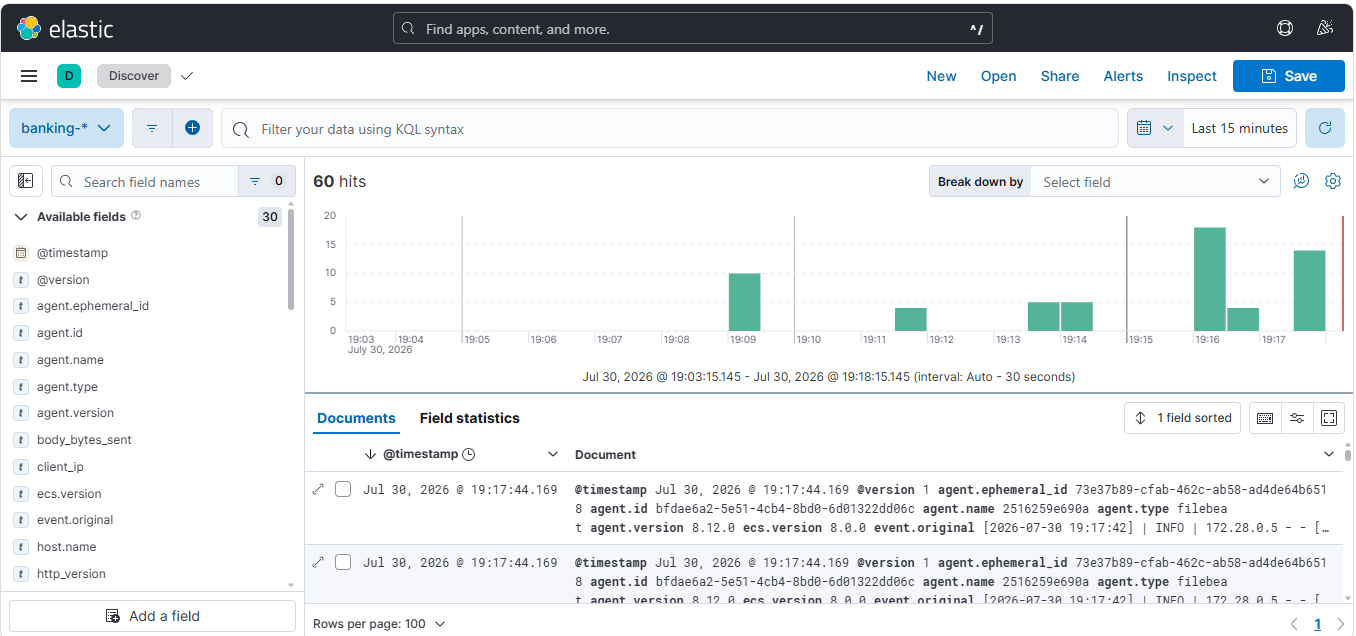
\includegraphics[width=1\linewidth]{uploads/SIEM_elk_elastic.png}
    \caption{Tableau de bord SIEM sous Kibana indexant les flux de sécurité NGINX, FastAPI et Keycloak.}
    \label{fig:app_siem_elk}
\end{figure}

Comme l'exhibe la Figure~\ref{fig:app_siem_elk}, les visualisations agrégées (cartes de répartition des IP sources, histogrammes de sévérité, distribution des codes d'erreur) fournissent à l'analyste une appréciation globale immédiate de la posture défensive.

La Figure~\ref{fig:app_siem_temps_reel} illustre la vue d'investigation en temps réel dans Kibana Discover.

\begin{figure}[H]
    \centering
    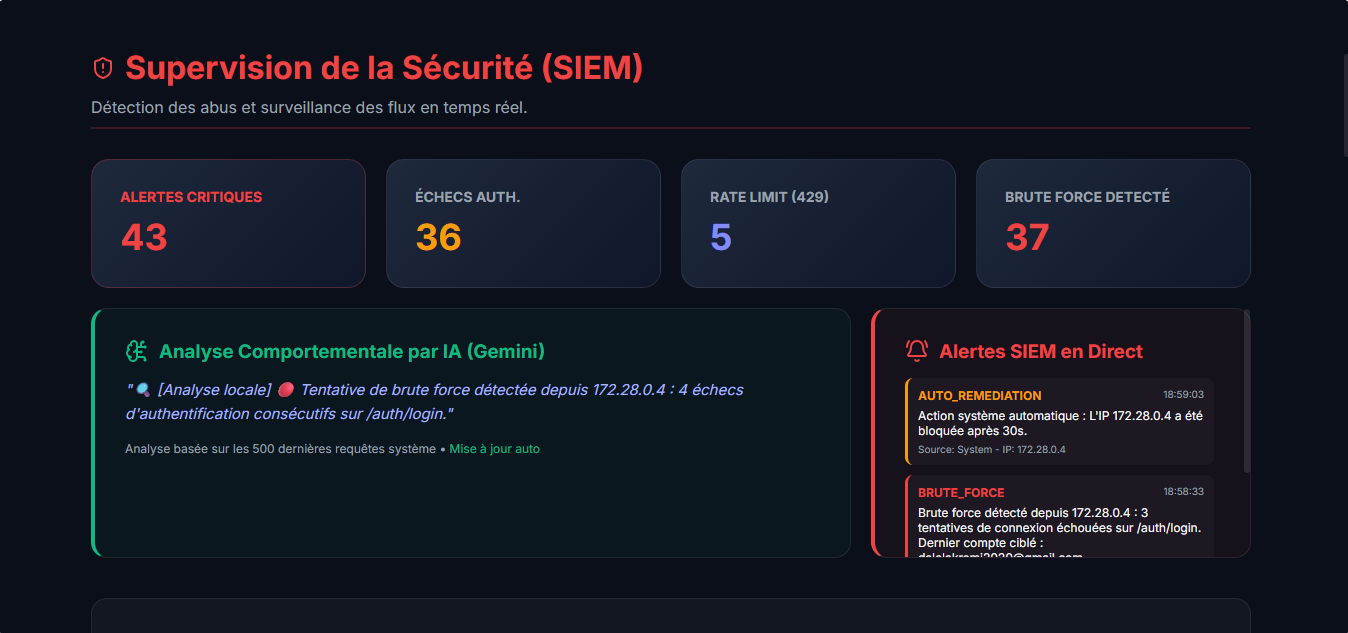
\includegraphics[width=1\linewidth]{uploads/SIEM_temps_reel.png}
    \caption{Interface de recherche en temps réel Kibana Discover avec filtres par niveau de sévérité et IP.}
    \label{fig:app_siem_temps_reel}
\end{figure}

L'interface présentée en Figure~\ref{fig:app_siem_temps_reel} constitue l'outil privilégié de recherche forensique pour investiguer les événements suspects ingérés au fil de l'eau.

\subsection{Synthèse de la conformité réglementaire et discussion critique}
La conformité du prototype aux cadres légaux et normatifs majeurs est résumée dans le Tableau~\ref{tab:compliance}.

\begin{table}[!htbp]
    \centering
    \small
    \begin{tabular}{|p{3.2cm}|p{3.8cm}|p{6cm}|}
        \hline
        \textbf{Réglementation} & \textbf{Exigence clé} & \textbf{Mise en œuvre technique démontrée} \\ \hline
        \textbf{PSD2 / DSP2 (SCA)} & Authentification forte du client & Combinaison mTLS (TPP), signature JWT asymétrique RS256 et second facteur OTP / TOTP. \\ \hline
        \textbf{PSD2 (Supervision)} & Détection et prévention de fraude & Pipeline SIEM temps réel avec calcul de score dynamique et remédiation autonome SOAR en $<$ 30s. \\ \hline
        \textbf{RGPD} & Confidentialité des données personnelles & Cloisonnement réseau Zero Trust, masquage du PAN et exclusion des données sensibles des journaux. \\ \hline
        \textbf{RGPD} & Auditabilité et intégrité & Journaux d'audit à altération détectable (format append-only horodaté) et indexation horodatée. \\ \hline
    \end{tabular}
    \caption{Synthèse de la gouvernance et de la conformité aux standards réglementaires.}
    \label{tab:compliance}
\end{table}

Ce Tableau~\ref{tab:compliance} confirme l'adéquation étroite entre les exigences juridiques du secteur bancaire et les solutions architecturales déployées. L'analyse critique de ces résultats met toutefois en relief certaines limites inhérentes au prototype : le filtrage applicatif en mémoire doit être migré vers une couche partagée Redis et des règles eBPF en production, tandis que l'évaluation du score de menace pourrait être enrichie par des modèles d'apprentissage non supervisé pour détecter des attaques lentes et distribuées (\textit{low and slow}).

\clearpage
% ============================================================
\section{Conclusion}
% ============================================================

Au terme de ce mémoire, nous avons conçu, réalisé et validé une architecture de sécurité \textit{Zero Trust} dédiée aux API bancaires ouvertes et conforme aux exigences de l'Open Banking et de la directive PSD2. En associant des technologies éprouvées --- une passerelle NGINX avec mTLS, un serveur d'identité Keycloak utilisant des jetons JWT signés avec RS256, un backend FastAPI, un frontend Flask et une pile de supervision ELK ---, le prototype démontre qu'il est possible d'assurer un cloisonnement rigoureux sans dégrader l'expérience utilisateur ni dépasser les contraintes opérationnelles.

L'apport principal de ce travail réside dans le passage d'un modèle de supervision passive à un système de défense réactive de type SOAR. Grâce à la modélisation formelle du score dynamique de menace $T_{decay}(x, t)$ et à la diffusion d'alertes en temps réel au moyen de Server-Sent Events, le prototype peut isoler automatiquement une source hostile en moins de 30 secondes, tout en maintenant le contrôle de l'analyste de sécurité. Les audits DAST réalisés avec OWASP ZAP n'ont révélé aucune vulnérabilité critique dans le périmètre évalué. Les mesures de performance indiquent un surcoût de latence de 34,1~ms et une latence totale de 72,3~ms, soit une valeur nettement inférieure au seuil SLA de 200~ms.

\subsection*{Perspectives}
Plusieurs axes d'évolution permettraient d'étendre la maturité de cette architecture vers un déploiement bancaire à grande échelle :
\begin{itemize}[leftmargin=*]
    \item \textbf{Décentralisation de l'état de sécurité via Redis et eBPF} : Migration du registre des adresses bloquées vers un cluster Redis partagé et injection automatique des règles de blocage au niveau noyau Linux via eBPF, assurant une protection à l'échelle du réseau.
    \item \textbf{Détection comportementale avancée} : Intégration de modèles d'apprentissage automatique non supervisé au sein d'Elasticsearch pour identifier des anomalies de navigation complexes et des fraudes de logique métier.
    \item \textbf{Certification PCI-DSS Niveau 1} : Extension des contrôles cryptographiques et de tokenisation pour couvrir l'intégralité du cycle de vie des données de cartes de paiement.
\end{itemize}

% ============================================================
\section*{Remerciements}
% ============================================================
Je tiens à exprimer ma profonde gratitude à toutes les personnes qui ont contribué, de près ou de loin, à l'aboutissement de ce travail de recherche et de développement.

Mes remerciements s'adressent tout particulièrement au corps professoral et à l'équipe pédagogique du Mastère Professionnel en Sécurité des Systèmes d'Information (MPSSI) de l'Institut Supérieur d'Informatique et de Multimédia de Gabès (ISIMG), Université de Gabès, pour la qualité de leur enseignement, leur disponibilité et les conseils méthodologiques prodigués tout au long de cette formation.

J'adresse également ma vive reconnaissance à \textbf{Mr. Akram Belazi} pour son encadrement attentif, ses remarques constructives et sa confiance constante durant les différentes phases de réalisation de ce projet.

Enfin, je remercie la communauté du logiciel libre et de la cybersécurité dont les outils ouverts et rigoureusement documentés --- NGINX, Keycloak, FastAPI, Docker, OWASP ZAP et la pile ELK --- ont constitué le socle technologique indispensable à la concrétisation de cette étude.